%%%%%%%%%%%%%%%%%%%%%%%%%%%%%%%%%%%%%%%%%%%%%%%%%%%%%%%%%%%%%%%%%%%%%%%%%%%%%%%%%%%
%%                                                                               %%
%% Document author: Moises Chavez-Martinez                                       %%
%%                                                                               %%
%% Description: This document is intended to be a technical and user manual for  %%
%%              the reader. In this document will be explained all the possible  %%
%%              details about the LibOpenCIF library.                            %%
%%                                                                               %%
%% --- Resources ---                                                             %%
%%                                                                               %%
%% This document is based on The Legrand Orange Book LaTex template:             %%
%% http://www.latextemplates.com/template/the-legrand-orange-book                %%
%%                                                                               %%
%% The icons used in the notes for the document (the Info, Warning               %%
%% and Error icons) where originally found at these sites:                       %%
%% http://www.iconsdb.com/green-icons/info-icon.html                             %%
%% http://www.iconsdb.com/orange-icons/warning-5-icon.html                       %%
%% http://www.iconsdb.com/red-icons/error-5-icon.html                            %%
%%                                                                               %%
%% Front cover image found at these sites:                                       %%
%% http://www.muycomputer.com/files/HIDDEN_264_19888_FOTO_Intel_4004_esquema.jpg %%
%% http://www.trecut.wellcome.ro/?p=3537                                         %%
%%                                                                               %%
%%%%%%%%%%%%%%%%%%%%%%%%%%%%%%%%%%%%%%%%%%%%%%%%%%%%%%%%%%%%%%%%%%%%%%%%%%%%%%%%%%%

%%%%%%%%%%%%%%%%%%%%%%%%%%%%%%%%%
%%                             %%
%% PREAMBLE AND FIRST COMMANDS %%
%%                             %%
%%%%%%%%%%%%%%%%%%%%%%%%%%%%%%%%%

\documentclass[11pt,twoside,openany,x11names,svgnames]{memoir}

\usepackage{lmodern}
\usepackage{wallpaper}
\usepackage{tikz}
\usepackage{listings}
\usetikzlibrary{shapes,positioning}

\usepackage[utf8]{inputenc}

\usepackage[english]{babel}
\selectlanguage{english} 

%% Custom stock paper and page size
\setstocksize{279mm}{216mm}
\settrimmedsize{\stockheight}{\stockwidth}{*}

%% Adjust margins around typeblock
\setlrmarginsandblock{23mm}{18mm}{*}
\setulmarginsandblock{23mm}{23mm}{*}

%% Header and footer heights
\setheadfoot{\baselineskip}{10mm}
\setlength\headsep{7mm}

%% To apply and enforce layout
\checkandfixthelayout

%% Command to hold chapter illustration image
\newcommand\chapterillustration{}

%% Define a fancy chapter style
\makechapterstyle{FancyChap}{
	%% Vertical Space before main text starts
	\setlength\beforechapskip{0pt}
	\setlength\midchapskip{0pt}
	\setlength\afterchapskip{137mm}
	%% Will print chapter number and title
	%% in one go ourselves
	\renewcommand*\printchaptername{}
	\renewcommand*\printchapternum{}
	%%% Re-define how the chapter title is printed
	\def\printchaptertitle##1{
		%% Background image at top of page
		\ThisULCornerWallPaper{1}{\chapterillustration}
		%% Draw a semi-transparent rectangle across the top
		\tikz[overlay,remember picture]
	  	\fill[fill=LimeGreen,opacity=.7]
			(current page.north west) rectangle 
			([yshift=-3cm] current page.north east);
		%% Check if on an odd or even page
		\strictpagecheck\checkoddpage
		%% On odd pages, "logo" image at lower right
		%% corner; Chapter number printed near spine
		%% edge (near the left); chapter title printed
		%% near outer edge (near the right).
		\ifoddpage{
		    \begin{tikzpicture}[overlay,remember picture]
			    \node[anchor=south west,
					xshift=20mm,yshift=-30mm,
					font=\sffamily\bfseries\huge] 
  	 	   			at (current page.north west) 
 	  	   			{\chaptername\chapternamenum\thechapter};
 	  	 		\node[fill=ForestGreen!80!black,text=white,
 	  	   			font=\Huge\bfseries, 
 	  	   			inner ysep=12pt, inner xsep=20pt,
 	     			rounded rectangle,anchor=east, 
 	     			xshift=-20mm,yshift=-30mm] 
 	     			at (current page.north east) {##1};
 		   	\end{tikzpicture}
 	 	}
	  	%% On even pages, "logo" image at lower left
  		%% corner; Chapter number printed near outer
  		%% edge (near the right); chapter title printed
  		%% near spine edge (near the left).
  		\else{
   	 		\begin{tikzpicture}[overlay,remember picture]
    			\node[anchor=south east,
      				xshift=-20mm,yshift=-30mm,
      				font=\sffamily\bfseries\huge] 
      				at (current page.north east)
      				{\chaptername\chapternamenum\thechapter};
    			\node[fill=ForestGreen!80!black,text=white,
      				font=\Huge\bfseries,
      				inner sep=12pt, inner xsep=20pt,
      				rounded rectangle,anchor=west,
      				xshift=20mm,yshift=-30mm] 
      				at ( current page.north west) {##1};
    		\end{tikzpicture}
  		}
  		\fi
	}
}


%% Define a fancy chapter style for unnumbered
%% chapters (e.g. the Table of Contents)
\makechapterstyle{FancyUnnumberedChap}{
	%% Vertical Space before main text starts
	\setlength\beforechapskip{0pt}
	\setlength\midchapskip{0pt}
	\setlength\afterchapskip{47mm}
	%% Will print chapter number and title
	%% in one go ourselves
	\renewcommand*\printchaptername{}
	\renewcommand*\printchapternum{}
	%%% Re-define how the chapter title is printed
	\def\printchaptertitle##1{
		%% Draw a semi-transparent rectangle across the top
		\tikz[overlay,remember picture]
	  	\fill[fill=LimeGreen,opacity=.7]
  			(current page.north west) rectangle 
			([yshift=-3cm] current page.north east);
  		%% Check if on an odd or even page
  		\strictpagecheck\checkoddpage
  		\ifoddpage{
    		\begin{tikzpicture}[remember picture, overlay]
    			\node[fill=ForestGreen!90!black,text=white,
    			font=\Huge\bfseries, 
    	  		inner ysep=12pt, inner xsep=20pt,
    	 	 	rounded rectangle,anchor=east, 
    			xshift=-20mm,yshift=-30mm] 
    	  		at (current page.north east) {##1};
    		\end{tikzpicture}
  		}
  		\else{
    		\begin{tikzpicture}[remember picture, overlay]
    			\node[fill=ForestGreen!80!black,text=white,
    	  			font=\Huge\bfseries,
     	 			inner sep=12pt, inner xsep=20pt,
     	 			rounded rectangle,anchor=west,
     	 			xshift=20mm,yshift=-30mm] 
     	 			at ( current page.north west) {##1};
    		\end{tikzpicture}
  		}
  		\fi
	}
}


%% Set the uniform width of the colour box
%% displaying the page number in footer
%% to the width of "99"
\newlength\pagenumwidth
\settowidth{\pagenumwidth}{99}

%% Define style of page number colour box
\tikzset{
	pagefooter/.style={
		anchor=base,font=\sffamily\bfseries\small,
		text=white,fill=YellowGreen!80!black,text centered,
		text depth=17mm,text width=\pagenumwidth
	}
}

%% Concoct some colours of our own
\definecolor[named]{GreenTea}{HTML}{CAE8A2}
\definecolor[named]{MilkTea}{HTML}{C5A16F}
\definecolor{charcoal}{rgb}{0.21, 0.27, 0.31}

%% Sometimes I prefer not to upper-case my
%% running headers
\nouppercaseheads

%% Re-define running headers on non-chapter odd pages
\makeoddhead{headings}
%% Left header is empty but I'm using it as a hook to paint the
%% background rectangles underneath everything else
{
	\begin{tikzpicture}[remember picture,overlay]
		\fill[MilkTea!25!white] (current page.north east) 
			rectangle (current page.south west);
		\fill[white, rounded corners] 
			([xshift=-10mm,yshift=-20mm]current page.north east) rectangle 	
			([xshift=15mm,yshift=17mm]current page.south west);
	\end{tikzpicture}}%
%% Blank centre header
{}%
%% Display a decorate line and the right mark (chapter title)
%% at right end
{
	\begin{tikzpicture}[xshift=-.75\baselineskip,yshift=.25\baselineskip,remember picture, overlay,fill=GreenTea,draw=GreenTea]\fill circle(3pt);\draw[semithick](0,0) -- (current page.west |- 0,0);\end{tikzpicture}\sffamily\itshape\small\rightmark
}

%% Re-define running footers on odd pages
%% i.e. display the page number on the right
\makeoddfoot{headings}{}{}{%
	\tikz[baseline]\node[pagefooter]{\thepage};
}
\makeoddfoot{plain}{}{}{\tikz[baseline]\node[pagefooter]{\thepage};}

%% Re-define running headers on non-chapter even pages
\makeevenhead{headings}
%% Draw the background rectangles; then the left mark (section
%% title) and the decorate line
{
	{
		\begin{tikzpicture}[remember picture,overlay]
			\fill[MilkTea!25!white] (current page.north east) rectangle (current page.south west);
			\fill[white, rounded corners] ([xshift=-15mm,yshift=-20mm]current page.north east) rectangle ([xshift=10mm,yshift=17mm]current page.south west);
		\end{tikzpicture}
	}%
	\sffamily\itshape\small\leftmark\ 
	\begin{tikzpicture}[xshift=.5\baselineskip,yshift=.25\baselineskip,remember picture, overlay,fill=GreenTea,draw=GreenTea]\fill (0,0) circle (3pt); \draw[semithick](0,0) -- (current page.east |- 0,0 );\end{tikzpicture}
}
{}
{}
\makeevenfoot{headings}{\tikz[baseline]\node[pagefooter]{\thepage};}{}{}
\makeevenfoot{plain}{\tikz[baseline]\node[pagefooter]{\thepage};}
%% Empty centre and right headers on even pages
{}
{}

%%%%%%%%%%%%%%%%%%%%%%%%%%%%%%%%%%%%%%%
%%                                   %%
%% PERSONAL DEFINITIONS AND COMMANDS %%
%%                                   %%
%%%%%%%%%%%%%%%%%%%%%%%%%%%%%%%%%%%%%%%

\lstdefinestyle{CPPStyle}
{
	belowcaptionskip=1\baselineskip,
	breaklines=true,
	frame=L,
	xleftmargin=\parindent,
	language=C++,
	showstringspaces=false,
	basicstyle=\footnotesize\ttfamily,
	keywordstyle=\bfseries\color{green!40!black},
	commentstyle=\itshape\color{purple!40!black},
	identifierstyle=\color{blue},
	stringstyle=\color{orange},
	numbers=left
}

\lstdefinestyle{SystemCommandStyle}
{
  belowcaptionskip=1\baselineskip,
  breaklines=true,
  xleftmargin=\parindent,
  showstringspaces=false,
  basicstyle=\footnotesize\ttfamily
}

\newcommand{\IconNote}[3]
{
	% Original icons:
	% http://www.iconsdb.com/green-icons/info-icon.html
	% http://www.iconsdb.com/orange-icons/warning-5-icon.html
	% http://www.iconsdb.com/red-icons/error-5-icon.html
	\begin{table}[ht]
	\begin{tabular}{ lm{\dimexpr\textwidth-8\tabcolsep-\wd0}@{}}
		\toprule
		\includegraphics[width=10mm, height=10mm]{images/icon-#1.png}
		&
		\parbox[t]{155mm}{
		\textbf{#2} \\
		#3
		}
	\end{tabular}
\end{table}
}

%%%%%%%%%%%%%%%%%%%%%%%%%%%%%%%%%%
%%                              %%
%% START OF THE DOCUMENT ITSELF %%
%%                              %%
%%%%%%%%%%%%%%%%%%%%%%%%%%%%%%%%%%

\begin{document}

%%%%%%%%%%%%%%%%%%%%%%%%%%%%%%%%%%%%%%%%%%%%%%%%%
%% These lines prevent a warning about spacing %%
%%%%%%%%%%%%%%%%%%%%%%%%%%%%%%%%%%%%%%%%%%%%%%%%%
\makeatletter
\edef\orig@output{\the\output}
\output{\setbox\@cclv\vbox{\unvbox\@cclv\vspace{0pt plus 20pt}}\orig@output}
\makeatother

\frontmatter

%% No header nor footer on the cover
\thispagestyle{empty}

%% Cover illustration
\ThisLLCornerWallPaper{1}{images/front-cover}

%% Bar across the top
\tikz[remember picture,overlay]%
\node[fill=ForestGreen,text=white,font=\LARGE\bfseries,text=Cornsilk,%
	minimum width=\paperwidth,minimum height=5em,anchor=north]%
	at (current page.north){Technical and user documentation};

\vspace*{2\baselineskip}

%%%%%%%%%%%%%%%%%%%%%%%%%
%%                     %%
%% DOCUMENT TITLE TEXT %%
%%                     %%
%%%%%%%%%%%%%%%%%%%%%%%%%

{
	\bfseries\itshape\color{charcoal}\fontsize{36pt}{46pt}\selectfont
		LibOpenCIF\par
		Complete manual\par}

\vspace*{2\baselineskip}

{\LARGE\color{charcoal}
Version 1.2.0\par}

\tikz[remember picture,overlay]%
\node[fill=ForestGreen,font=\LARGE\bfseries,text=Cornsilk,%
	minimum width=\paperwidth,minimum height=3em,anchor=south]%
 	at (current page.south) {};

\begin{center}
\LARGE\bfseries\color{SaddleBrown!30!black}

\end{center}

\cleartorecto

%%%%%%%%%%%%%%%%%%%%%%%
%%                   %%
%% TABLE OF CONTENTS %%
%%                   %%
%%%%%%%%%%%%%%%%%%%%%%%

%% Invoke fancy unnumbered chapter style
%% for the table of contents
\chapterstyle{FancyUnnumberedChap}
\renewcommand{\contentsname}{Contents}
\setcounter{tocdepth}{3}
\tableofcontents*

%% Main matter starts here; resets page-numberings to arabic numeral 1
\mainmatter

%% Invoke the FancyChap chapter style
\chapterstyle{FancyChap}

\setcounter{secnumdepth}{2}

\renewcommand\chapterillustration{images/chapter01-cover}
\renewcommand{\chaptername}{Chapter}
\renewcommand{\figurename}{Figure}

%%%%%%%%%%%%%%%%%%%%%%%%%%%%%%%%%%%%%%%%%%
\chapter{Introduction}\label{Introduction}
%%%%%%%%%%%%%%%%%%%%%%%%%%%%%%%%%%%%%%%%%%

In this chapter, the user will learn the background needed to understand crucial concepts related to the usage of this library. Some of these concepts are basic definitions of what is a CIF file and what is a library.

Also, there is recommended that the user takes the time to read this chapter, since here is explained how the contents are organized and how the information is provided (for example, is explained how to identify a command and how to read the example code).
\newpage 

%%%%%%%%%%%%%%%%%%%%%%%%%%%%%%%%%%%%%%%%%%%%%%%%%%%%%%%%%%%%%%%%%%%%%%%%%
\section{Who must read this document?}\label{Who-must-read-this-document}
%%%%%%%%%%%%%%%%%%%%%%%%%%%%%%%%%%%%%%%%%%%%%%%%%%%%%%%%%%%%%%%%%%%%%%%%%

This document is intended to be read by any user that needs to read a CIF file and wants or need to understand how to use the LibOpenCIF library. This document makes big assumptions about the reader. One of the most important is that the reader must be already aware and is familiarized with the concepts related to integrated circuit designs, what are they and what is a layout.

Also, is important to note that this document is intended to be read by a user that already has knowledge about how to program in the C++ language, since will not be explained, for example, what is a class, what is a variable, what is a class instance, and other core concepts of the Object Oriented Programming. This is the reason that this document might be easier to read for a programmer rather than a specialist in circuit design.

Finally, in this document we assume that the user is already familiarized with the use of the operative system on which is desired to use the library. Among other operations, the user must be already capable of opening a terminal emulator, run commands on it, move itself between folders using commands and manipulate files using a file viewer (like Explorer on Microsoft Windows systems, Dolphin or Nautilus on GNU/Linux systems or Finder on Apple Mac OS X systems).

%%%%%%%%%%%%%%%%%%%%%%%%%%%%%%%%%%%%%%%%%%%%%%%%%%%%%%%
\section{What is a CIF file?}\label{What-is-a-CIF-file}
%%%%%%%%%%%%%%%%%%%%%%%%%%%%%%%%%%%%%%%%%%%%%%%%%%%%%%%

The first concept that is needed to understand this document is the definition of what a CIF file is. This definition is critical to comprehend the whole idea behind the library and its functionality.

The \textbf{CIF} acronym comes from the name \textbf{Caltech Intermediate Form}, and it defines a very specific format used to represent and store the \textit{layout} of an \textbf{integrated circuit design}. In other words, a CIF file describes \textit{how a circuit design looks}. Such description is achieved using two-dimensional figures, like rectangles, circles and polygons.

All of the information related to the circuit is stored in a \textit{\textbf{plain text file}} using \textit{\textbf{commands}}. The commands can be \textit{instructions}, \textit{figures} or \textit{expansion commands}.

The instruction commands are used to control how the circuit is being defined. For example, they are used to instruct the reader where a definition of a \textit{cell} starts and ends, and when is being used. A figure command can define a visual component of the design, such a rectangle, its position, size and rotation. And finally, the expansion commands are special commands that the CIF format allows to be user-defined. This means that the reader of the file can interpret the command in a specific way, expanding the capabilities of the format, allowing the user to define things that where not originally intended to be supported, like cell names, node definitions, among others.

In the industry, various file formats exists that are intended to do the same thing: store integrated circuit designs. Along with the CIF format, there exists other popular formats to store designs. Of course, there are differences between formats, and every one has its advantages and disadvantages. Some files store the information in binary format (making the information very complex to read by a human, but easier to manage by a machine), others, like the CIF format, store the information in plain text (making the information easier to read by humans and making the format more flexible about its contents, but the information becomes more complex to read and manage by a machine).

%%%%%%%%%%%%%%%%%%%%%%%%%%%%%%%%%%%%%%%%%%%%%%%%%%%%%%%
\section{What is LibOpenCIF?}\label{What-is-LibOpenCIF}
%%%%%%%%%%%%%%%%%%%%%%%%%%%%%%%%%%%%%%%%%%%%%%%%%%%%%%%

LibOpenCIF is a C++ library intended to help the users with the task of reading and validating the contents of a CIF file into memory. The library is intended to be used in various operating systems, like GNU/Linux, Microsoft Windows and Apple Mac OS X.

For GNU/Linux and Mac OS X systems, the library can be compiled and installed into the system. After that, will be available as a static library. This means that any program compiled with it will be able to run even if the library is uninstalled from the system. This is also due to the fact that the library is very small.

For Microsoft Windows (and, in general, for all the systems if needed) the library has a two-file presentation. This means that, instead of compiling the library into a DLL file, can be added directly to the file structure of programs as a regular piece of code (a source and header files are included). This means that all kinds of projects in C++ can use the library. This presentation is intented to help Microsoft Windows users, and also, if required, be of use for other systems.

%%%%%%%%%%%%%%%%%%%%%%%%%%%%%%%%%%%%%%%%%%%%%%%%%%%%%%%%%%%%%
\section{Why create LibOpenCIF?}\label{Why-create-LibOpenCIF}
%%%%%%%%%%%%%%%%%%%%%%%%%%%%%%%%%%%%%%%%%%%%%%%%%%%%%%%%%%%%%

The original author of the library, Moises Chavez-Martinez, worked in various projects related to the process of design of integrated circuits. In all of those projects, the files used to store the designs were in CIF format. Working on applications that were made from the ground up, the lack of open utilities to read the CIF files became a reality, making really hard the process of reading the contents of such files, especially the process of validating the commands of the files (more of this in later sections).

The author decided to create a very specific library in C++ that can help him and other people writing and upgrading its own applications. The author decided that his work might be of help for others, and so, released his work as Open Source.

%%%%%%%%%%%%%%%%%%%%%%%%%%%%%%%%%%%%%%%%%%%%%%%%%%%%%%%%%%%%%%%%%%%%%%%%%%%%%%%%%%
\section{What can and can't do LibOpenCIF?}\label{What-can-and-cant-do-LibOpenCIF}
%%%%%%%%%%%%%%%%%%%%%%%%%%%%%%%%%%%%%%%%%%%%%%%%%%%%%%%%%%%%%%%%%%%%%%%%%%%%%%%%%%

The LibOpenCIF library is intended to be able to:

\begin{itemize}
	\item Open a desired CIF file.
	
	\item Try to load its contents, validating them using a specialy designed Finite State Machine.
	
	\item Clean and format the contents of the file loaded into easy-to-process strings.
	
	\item Convert the commands loaded (in string form) into instances of special classes provided.
	
	\item Provide a manual or full-automatic loading process.
	
	\item Be partialy relaxed or completely strict when validating the contents of the file.
\end{itemize}

Also, the library can provide to the user these next services, being them not directly intented to:

\begin{itemize}
	\item If the input file has the expected format, the user can read its contents directly into memory using class instances.\footnote{There is no automatic detection of which command is going to be loaded, that is a task left to the user. So, when using this capability, the user needs to know in advance which command is going to be the next, so he can use the correct class instance.}
	\item The class instances can write their contents into a file, allowing the user to write CIF files using configured class instances.
	\item Is possible to validate commands (in string form).
	\item Is possible to clean commands (in string form).
\end{itemize}

Finally, the library isn't intented to provide these services, since they are beyond the original scope of the design:

\begin{itemize}
	\item The library will never convert values into floating point representations.\footnote{The values on an integrated circuit design, by definition, need floating point values for positions and sizes. Since those values are very important, and any error related to precision can affect negatively a design, the CIF format doesn't handle directly those values. In exchange, the format manages all of those values using \textbf{\textit{fractions}}, making the values error-less and leaving the convertion and precision in hands of the reader.} All of the values found in the input file will be stored and provided to the user in form of fractions.
	\item Validation of the design stored (looking for missing commands, logical errors, unused cells, cyclic calls, etc). The library is intented only to load and validate the commands, not the structure of the design. That is a task for which the user is responsible.
\end{itemize}

%%%%%%%%%%%%%%%%%%%%%%%%%%%%%%%%%%%%%%%%%%%%%%%%%%%%%%%
\section{Why use LibOpenCIF?}\label{Why-use-LibOpenCIF}
%%%%%%%%%%%%%%%%%%%%%%%%%%%%%%%%%%%%%%%%%%%%%%%%%%%%%%%

There are various reasons why you can choose LibOpenCIF above other solutions to load a CIF file:

\begin{itemize}
	\item The library is Open Source. You are not expected to pay any royalty for the usage of the library. Being released as GPL software, you just need to give credit to the original author.
	\item You can customize and extend the library. If the library can do more for you, and you know how to extend the library, then you can do it. Being released under the GPL license means that you can modify and extend the library as much as you want. You just need to give the proper credits to the original author.
	\item You will not need to implement this complex task by yourself. Most of the public projects that manage circuit designs in CIF format (Open Source or private) use their own routines to load the contents of the files. If you are starting a new project, you can have this library as a starting point.
	\item Easy to use. The library was designed to be as simple as possible.
	\item Portable. The library is programmed using pure standard C++. That means that you will not need external libraries to compile it, making the library platform independant.
\end{itemize}

%%%%%%%%%%%%%%%%%%%%%%%%%%%%%%%%%%%%%%%%%%%%%%%%%%%%%%%%%%%%%%%%
\section{The library can be used in other programing languages?}\label{The-library-can-be-used-in-other-programming-languages}
%%%%%%%%%%%%%%%%%%%%%%%%%%%%%%%%%%%%%%%%%%%%%%%%%%%%%%%%%%%%%%%%

Is expected to be released a new library version for other major languages, since it has been ported to other languages, like Java, C and Python.

%%%%%%%%%%%%%%%%%%%%%%%%%%%%%%%%%%%%%%%%%%%%%%%%%%%%%%%%
\section{About this document}\label{About-this-document}
%%%%%%%%%%%%%%%%%%%%%%%%%%%%%%%%%%%%%%%%%%%%%%%%%%%%%%%%

Is expected that the user reads all the contents of this document, and even in that case, the themes are ordered in incremental order. There are the contents expected to be covered in this document:

\begin{itemize}
	\item Chapter 2 (User documentation): In this chapter, the user will learn basic aspects of the usage of the library, from how to install and uninstall it, to how to compile and use the capabilities provided in example programs. All of the themes covered are platform independent, exept for the ones related to how to install, uninstall and compile (examples for every major operative system considered are provided).
	\item Chapter 3 (Technical documentation): In this chapter, the user will learn advanced topics related to the operation and design of the library. Among other themes, will be explained in detail how the library loads and validates the contents of the files (complete Finite State Machine included), how the commands are cleaned, the reasons behind the design desicions and a complete UML map of the classes and their relations.
\end{itemize}

In the document, when speaking about code, the reader can expect to see sections like this one:

\lstinputlisting[caption={Example program}, style=CPPStyle]{examples/chapter1-example1.cc}

In the previous example, you can see how the code will look once an example is provided to you. The code is in C++ (most of the examples in this document will be about C++ code). The code examples are intended to be stored in plain text files. Those code files can have various filename extentions, depending if they are source or header files. Some of the supported file extentions for C++ source files are \textbf{.cc, .C,} and \textbf{.cpp}. All of them are valid (the second one has the problem of being easily confused with a C language source code file). In this document, we will be using the \textbf{.cc} file extention for source files, and the \textbf{.hh} file extention for the header files (instead of the popular \textbf{.hpp} used by some projects). 

In this document, you will also find system commands. Those system commands are intented to be entered and executed in terminal emulators. In GNU/Linux, Apple Mac OS X and similar systems, some examples of those systems are Konsole, Gnome Terminal, XTERM and Terminal. In Microsoft Windows systems, there are, at least, two options to use by the reader: the Windows CMD or Windows PowerShell are the most common choices on terminals on these systems.

When needed, there will be shown to the user system commands. The next is an example of a command for GNU/Linux, Apple Mac OS X or similar systems:

\begin{lstlisting}[frame=single,style=SystemCommandStyle]
$ cd /mnt/
$ ls
Disk1   Disk2   Disk3   Disk4
$
\end{lstlisting}

The previous example shows how a command can be executed and some of the output. These commands can be identified as intended as to be executed in GNU/Linux or similar systems because the commands start with a \textbf{\$} character. Such character is commonly used in terminal emulators of these systems. The next command example is for Microsoft Windows systems:

\begin{lstlisting}[frame=single,style=SystemCommandStyle]
> cd C:\Windows\System32\
> 
\end{lstlisting}

The previous example shows how a command can be exeucted for Microsoft Windows systems. These commands can be identified as to be executed in such systems because the command starts with a \textbf{\textgreater} character. Such caracter is commonly used in terminals of these systems.

Finally, in this document, the reader will find some special notes intended to help understanding some special concepts or critical information. The next boxes take care of various information types:

\IconNote
	{info}
	{This is an information message}
	{When reading this document, the reader is recommended to pay attention to these messages, since these may contain non-critical information, like reminders about important paths or recommended usages about the library components.}

\IconNote
	{warning}
	{This is a warning message}
	{When reading this document, the reader is expected to pay attention to these messages, since these may contain information about important details that might cause problems if ignored, like possible errors, common mistakes and more.}

\IconNote
	{error}
	{This is a critical or error message}
	{When reading this document, the reader is expected to pay special attention to these messages, since these may contain information about critical errors and mistakes that might affect in a very negative way your work.}

%%%%%%%%%%%%%%%%%%%%%%%%%%%%%%%%%%%%%%%%%%%%%%%%%%
\section{About the author}\label{About-The-Author}
%%%%%%%%%%%%%%%%%%%%%%%%%%%%%%%%%%%%%%%%%%%%%%%%%%
 
The author of this document is Moises Chavez-Martinez. He is a Computer Engineer with specialization on Systems Software from the Universidad de Guadalajara, in M\'exico. He is an enthusiast of the Open Source and likes to share his work.

During his career, he has worked in various professional applications aimed to help the task of designing Integrated Circuits. This granted him some knowledge of this work area, and shown him some deficiencies related to the work of applications for this industry area.

\renewcommand\chapterillustration{images/chapter02-cover}
%%%%%%%%%%%%%%%%%%%%%%%%%%%%%%%%%%%%%%%%%%%%%%%%%%%%%%
\chapter{User documentation}\label{User-documentation}
%%%%%%%%%%%%%%%%%%%%%%%%%%%%%%%%%%%%%%%%%%%%%%%%%%%%%%

In this chapter, the reader will learn all the concepts and procedures needed to understand how to install, uninstall and use the library in various operating systems. Among other details, will be discussed:

\begin{itemize}
	\item How to compile the source code in GNU/Linux and Mac OS X to create a static library.
	
	\item How to install the previously compiled static library.
	
	\item How to uninstall the installed library.
	
	\item How to compile a program using the library in all three major operative systems, in its two-file file mode and as a static library (mode available only on non-Windows systems).
	
	\item How to open a CIF file using the library.
	
	\item How to load the contents of a CIF file in a manually and fully automated way.
	
	\item How to use the information provided by the library once a file is loaded (a vector of strings or a vector of class instances).
\end{itemize}
\newpage 

%%%%%%%%%%%%%%%%%%%%%%%%%%%%%%%%%%%%%%%%%%%%%%%%%%%%%%%%%%%%%%
\section{Installing the library}\label{Installing-The-Library}
%%%%%%%%%%%%%%%%%%%%%%%%%%%%%%%%%%%%%%%%%%%%%%%%%%%%%%%%%%%%%%

The installation procedure is used only when a static library is needed, and such version is intended to be used only on the GNU/Linux and Apple Mac OS X systems. The library  is not intended to be installed on Microsoft Windows systems, since in such systems the library must be used as a two-file part of the reader's project (see section \ref{Compiling-On-Windows} to learn how to compile a project using the library).

These installation steps are intended to be used with the source version of the library. If the reader already have a pre-compiled version (as static or dinamic library), follow its specific steps to install the library.

To being able to install the library, the reader need to have some components before starting.

The first element is a package with the source code of the library. The needed file has a name like \textbf{\texttt{libopencif-X.Y.Z.tar.gz}}, where \textbf{\texttt{X}}, \textbf{\texttt{Y}} and \textbf{\texttt{Z}} are the major, minor and patch version numbers of the library. Is recommended to always look for the latest version of the library at SourceForge\footnote{https://sourceforge.net/projects/libopencif/} or GitHub\footnote{https://github.com/Tuxman88/LibOpenCIF/}.

The next component needed is a compiler. The recommended compiler is \textbf{GCC v4.8.0} or newer (with its C++ module installed). The easiest way to know if the needed compiler is installed is opening a terminal emulator (like Konsole, Gnome Terminal or XTERM in GNU/Linux systems or Terminal in Apple Mac OS X systems) and executing this command:

\begin{lstlisting}[frame=single,style=SystemCommandStyle]
$ g++
g++: fatal error: no input files
compilation complete.
$
\end{lstlisting}

As can be seen, the idea is to open a terminal emulator and run the command \textbf{\texttt{g++}} to see the output. If the compiler is installed, the reader must see an output similar to the one in the previous example. If the reader sees an output like this one:

\begin{lstlisting}[frame=single,style=SystemCommandStyle]
$ g++
bash: g++: command not found
$
\end{lstlisting}

Then the GCC compiler is not installed. In such case, please, follow the specific instructions of the reader's system to install the program.

After the compiler is installed and ready, the next application needed is \textbf{CMake v2.6} or newer. In a similar way, to check if it is installed, the command \textbf{\texttt{cmake}} can be executed and its output checked. If the reader see lots of text, then the application is installed (the output is a help message from the utility). But, if an output like this can be seen:

\begin{lstlisting}[frame=single,style=SystemCommandStyle]
$ cmake
bash: cmake: command not found
$
\end{lstlisting}

Then the application is not installed. Again, please, follow the specific steps in the reader's system to install the utility.

After these steps, everyting that is needed to compile and install the library is ready.

The first step is to extract the contents of the source package into a folder. To extract the contents of the package, run this command in the folder on which the package file is:

\begin{lstlisting}[frame=single,style=SystemCommandStyle]
$ tar -zxvf libopencif-X.Y.Z.tar.gz
...
$
\end{lstlisting}

After running the command (replace the \textbf{\texttt{X}}, \textbf{\texttt{Y}} and \textbf{\texttt{Z}} characters with the numbers of the version downloaded), a new folder named \textbf{\texttt{libopencif-X.Y.Z}} will be created.

Enter to the new folder and create a new folder inside named \textbf{\texttt{build}}.

Now, enter such new folder and run this command inside:

\begin{lstlisting}[frame=single,style=SystemCommandStyle]
$ cmake ..
\end{lstlisting}

After running the command, an output like this can be seen:

\begin{lstlisting}[frame=single,style=SystemCommandStyle]
$ cmake ..
-- The C compiler identification is GNU 4.9.2
-- The CXX compiler identification is GNU 4.9.2
-- Check for working C compiler: /usr/lib64/ccache/cc
-- Check for working C compiler: /usr/lib64/ccache/cc -- works
-- Detecting C compiler ABI info
-- Detecting C compiler ABI info - done
-- Check for working CXX compiler: /usr/lib64/ccache/c++
-- Check for working CXX compiler: /usr/lib64/ccache/c++ -- works
-- Detecting CXX compiler ABI info
-- Detecting CXX compiler ABI info - done
-- Configuring done
-- Generating done
-- Build files have been written to: /home/user/libopencif-1.2.1/build
$
\end{lstlisting}

\IconNote
	{info}
	{Compilling in 32 bit and 64 bit systems}
	{As can be noticed, the command output in the example displays some references to \textbf{\texttt{lib64}}. Such references can be different if the reader is compiling for a 32 bit system (these examples where captured in a 64 bit machine).}

After running the command, run this new one in the same folder:

\begin{lstlisting}[frame=single,style=SystemCommandStyle]
$ make
\end{lstlisting}

Now, the reader will be able to see output like this one (the example is not complete):

\begin{lstlisting}[frame=single,style=SystemCommandStyle]
$ make
Scanning dependencies of target opencif
[  3%] Building CXX object CMakeFiles/opencif.dir/src/command/command.cc.o
[  7%] Building CXX object CMakeFiles/opencif.dir/src/command/controlcommand/controlcommand.cc.o
...
[ 96%] Building CXX object CMakeFiles/opencif.dir/src/finitestatemachine/ciffsm.cc.o                                                                                                                                                         
[100%] Building CXX object CMakeFiles/opencif.dir/src/command/controlcommand/endcommand/endcommand.cc.o                                                                                                                                      
Linking CXX static library libopencif.a                                                                                                                                                                                                      
[100%] Built target opencif
$
\end{lstlisting}

\IconNote
	{warning}
	{Compilation errors}
	{The library must be error-free for compilation (not even warning messages should appear). If any error is found, please contact with the author of the library (see section \ref{About-The-Author}).}

The reader will now be able to install the library into its system. Run the following command and, when prompted, enter your user password to gain temporal root access:

\begin{lstlisting}[frame=single,style=SystemCommandStyle]
$ sudo make install
\end{lstlisting}

After running the command, the reader should see an output like this one:

\begin{lstlisting}[frame=single,style=SystemCommandStyle]
$ sudo make install
Password:
[100%] Built target opencif
Install the project...
-- Install configuration: ""
-- Installing: /usr/local/lib/libopencif.a
-- Installing: /usr/local/include/opencif
$
\end{lstlisting}

\IconNote
	{warning}
	{Installation errors}
	{If the reader finds any installation error, read carefully the output of the command to check for trivial problems. If the errors can't be solved by the reader, please, contact the author of the library (see section \ref{About-The-Author}).}

After the previous command, the library is expected to be correctly installed in the reader's system.

\IconNote
	{info}
	{Files and folders installed}
	{The installation is done by the CMake utility. It decides the paths where all the components will be installed. By default, it installs the static library in the path \textbf{\texttt{/usr/local/lib/}}, and the header file in the path \textbf{\texttt{/usr/local/include/}}.}
	
\IconNote
	{info}
	{Different paths}
	{The installation paths might be different in the reader's system. When installing, is recommended to check and store the paths used by CMake to install the library for later use when uninstalling.}

%%%%%%%%%%%%%%%%%%%%%%%%%%%%%%%%%%%%%%%%%%%%%%%%%%%%%%%%%%%%%%%%%%
\section{Uninstalling the library}\label{Uninstalling-the-library}
%%%%%%%%%%%%%%%%%%%%%%%%%%%%%%%%%%%%%%%%%%%%%%%%%%%%%%%%%%%%%%%%%%

The process of uninstalling the LibOpenCIF library is intended to be performed only by GNU/Linux and Apple Mac OS X users. This is due to the fact that the library is not installable on Microsoft Windows systems.

\IconNote
	{error}
	{Using commands as root}
	{Be careful when using commands as the root user, specially in this section since the procedures explained might require deleting files and folders recursively.}

The uninstall process only requires removing the installed files of the system. Since this process requires root access, is recommended to do this operation using commands, or, if the user has file navigators with root access, can use them to ease the process.

The first element to remove from the system is the library file itself. By default, the file can be found in the folder \textbf{\texttt{/usr/local/lib/}}. The file name must be \textbf{\texttt{libopencif.a}}. Using a terminal emulator, the reader can use these commands to go to the desired folder and remove the file:

\begin{lstlisting}[frame=single,style=SystemCommandStyle]
$ cd /usr/local/lib
$ ls
libopencif.a
$ sudo rm libopencif.a
Password:
$
\end{lstlisting}

\IconNote
	{warning}
	{Using commands with sudo}
	{Remember: When using commands with \textbf{sudo}, the password might be asked just the first time. After that, the current opened terminal is granted with a short period of time on which the password is no longer needed.}

\IconNote
	{info}
	{Deleting the library file}
	{When removing the library file, remove it directly (using the full file name). Is not recommended to use wildcards, since in the folder might be files with similar names.}

As can be seen, the \textbf{\texttt{ls}} command was used to see the contents of the folder and see if the file is there.

After deleting the library file, the next and last component to remove is the header file.  By default, the file can be found in the path \textbf{\texttt{/usr/local/include/}}. There can be found a file named \textbf{\texttt{opencif}}. To remove the file, use these commands:

\begin{lstlisting}[frame=single,style=SystemCommandStyle]
$ cd /usr/local/include
$ ls
opencif
$ sudo rm opencif
Password:
$
\end{lstlisting}

After running the \textbf{\texttt{rm}} command as root, the system might ask you if you really want to remove the file. Answer yes (since it is no longer needed).

If the previous steps were performed correctly and none error was found, the library was completely and successfuly uninstalled from your system.

%\begin{figure}
%	\centering
%	\label{fig:union-pn}
%	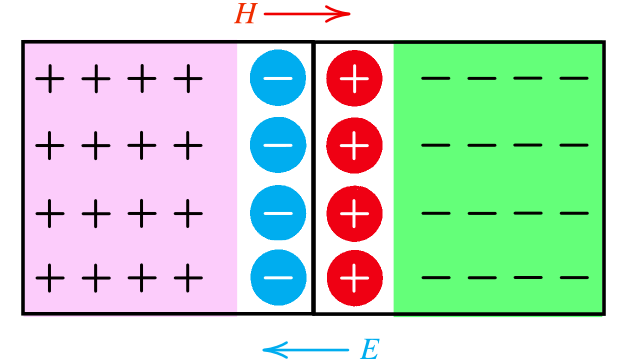
\includegraphics[scale=0.35, clip=true, trim= 0pt 0pt 0pt 0pt]{images/chapter02-image01}
%	\caption{Some figure.}
%\end{figure}

%%%%%%%%%%%%%%%%%%%%%%%%%%%%%%%%%%%%%%%%%%%%%%%%%%%%%%%%%%%%%%%%%%%%%%%%%
\section{Compiling a program with the library}\label{Compiling-a-program}
%%%%%%%%%%%%%%%%%%%%%%%%%%%%%%%%%%%%%%%%%%%%%%%%%%%%%%%%%%%%%%%%%%%%%%%%%

In this section, the reader will learn how to compile a program with LibOpenCIF support. Such procedure can vary depending on two factors:

\begin{itemize}
	\item Operating system used.
	\item Library mode used (static pre-compiled or two-file version).
\end{itemize}

In the next sub-sections, the reader will learn how to compile an example program in Microsoft Windows, GNU/Linux and Apple Mac OS X using the pre-compiled or two-file version of the library.

%%%%%%%%%%%%%%%%%%%%%%%%%%%%%%%%%%%%%%%%%%%%%%%%%%%%%%%%%%
\subsection{Microsoft Windows}\label{Compiling-On-Windows}
%%%%%%%%%%%%%%%%%%%%%%%%%%%%%%%%%%%%%%%%%%%%%%%%%%%%%%%%%%
 
For Microsoft Windows systems, the compilation can be done only in one way\footnote{The library is not intended to be pre-compiled on Microsoft Windows systems. If the reader finds a guide on how to pre-compile the library into, for example, a DLL file, then the reader will be the only responsible of the success of such alternatives. The author will not provide support on non-official compilation methods.}: Using the two file version of the library.

To get access to the two-file version of the library, the reader can download the regular source package of the library found in SourceForge or GitHub (see section \ref{Installing-The-Library} to find the URLs on which the package can be found). The downloaded file must be named \textbf{\texttt{libopencif-X.Y.Z.tar.gz}}, where \textbf{\texttt{X}}, \textbf{\texttt{Y}} and \textbf{\texttt{Z}} are the major, minor and patch version numbers of the package. Is recommended to always download the latest version of the library.

After getting the source package, uncompress it on your system (the reader can use various applications to extract the contents of a \textbf{\texttt{tar.gz}} file on these systems, like 7-ZIP). Enter the new folder created after the uncompress process and look for the folder named \textbf{\texttt{two-file}}. Such folder must contain two files: \textbf{\texttt{libopencif.cc}} and \textbf{\texttt{libopencif.hh}}. Those two files are the only files needed for Microsoft Windows systems.

By default, those two files of the library requires to be together all the time, since the source file (the \textbf{\texttt{.cc}} file) has an \textbf{\texttt{include}} statement calling the header file (the \textbf{\texttt{.hh}} file). If you require to use a different structure on the files, like placing the source and header files in different folders, you can edit the source file and change the include path. Such instruction can be found right after the GNU license preamble in line 24, approximately.

From this point, we are assuming that the reader has already a compilation mechanism in the intended system. In the case of the next examples, we use the MinGW\footnote{The installer can be found at \textbf{http://sourceforge.net/projects/mingw/files/Installer/}.} compiler for Microsoft Windows, being executed in a PowerShell window of Microsoft Windows 8.

For the next example, we created a temporal folder named \textbf{test1} in our \textbf{My Documents} path. Inside such folder, we copied the two files of the library and created a new file named \textbf{main.cc}. After the creation of the new file, the folder ended with these contents:

\begin{lstlisting}[frame=single,style=SystemCommandStyle]
> dir


    Directory: C:\Users\User\Documents\Projects\test1


Mode                LastWriteTime     Length Name
----                -------------     ------ ----
-a---     03/01/2015  08:57 p. m.      79037 libopencif.cc
-a---     03/01/2015  08:57 p. m.      31588 libopencif.hh
-a---     03/01/2015  09:57 p. m.        149 main.cc
>
\end{lstlisting}

Having all the needed files in place, the next step is to compile the library source file into object code. This is done using the next command:

\begin{lstlisting}[frame=single,style=SystemCommandStyle]
> g++ -c .\libopencif.cc
>
\end{lstlisting}

The previous command will instruct GCC to compile the source file of the library into object code. After calling this command, a new file will appear, named \textbf{\texttt{libopencif.o}}. Then, open your \textbf{\texttt{main.cc}} file and add this example code:

\lstinputlisting[caption={Include statement for Microsoft Windows the two-file version of the library.}, style=CPPStyle]{examples/chapter2-example1.cc}

As can be noticed, in line 2 can be found an include statement looking for the header file of the library. After adding the code and saving the changes, the reader can compile the whole program using this command:

\begin{lstlisting}[frame=single,style=SystemCommandStyle]
> g++ .\main.cc -o main.exe libopencif.o
>
\end{lstlisting}

The previous command will instruct GCC to compile the file \textbf{\texttt{main.cc}}, create the output binary file \textbf{\texttt{main.exe}} and add the object code found in the file \textbf{\texttt{libopencif.o}}.

After running the previous command, a new file can be found named \textbf{\texttt{main.exe}}. That file is the executable binary of our example program. To run the program in the terminal, use this command:

\begin{lstlisting}[frame=single,style=SystemCommandStyle]
> .\main.exe
LibOpenCIF: Example about compilation.
>
\end{lstlisting}

If the output of the command is as expected, then, the compilation process were done correctly.

%%%%%%%%%%%%%%%%%%%%%%%%%%%%%%%%%%%%%%%
\subsection{GNU/Linux}\label{GNU-Linux}
%%%%%%%%%%%%%%%%%%%%%%%%%%%%%%%%%%%%%%%

In GNU/Linux, the reader has two options to include the library into his project. The first option is using the static library after installing it in the system. The second option is using the two-file version of the library.

\IconNote
	{info}
	{Best usage method}
	{The recommended usage method for the library is installing the library, and then, linking your program with the static library. However, the reader is free to use the two-file version of the library. There is no major difference when using one option or another.}
	
%%%%%%%%%%%%%%%%%%%%%%%%%%%%%%%%%%%%%%%%%%%%%%%%%%%%%%%%%%%%%%%%%%%%%%%%%%%%%%
\subsubsection{Using the installed library}\label{Using-the-installed-library}
%%%%%%%%%%%%%%%%%%%%%%%%%%%%%%%%%%%%%%%%%%%%%%%%%%%%%%%%%%%%%%%%%%%%%%%%%%%%%%
	
To use the first option, the installed library, you first need to install the library. To do so, the reader needs to follow the steps found in the section \ref{Installing-The-Library}.

From this point, we are assuming that the reader has already a compilation mechanism in the intended system. In the case of the next examples, we use the GCC compiler (with its C++ module) for GNU/Linux, available in most GNU/Linux distributions, being executed in a Konsole terminal emulator, running Bash on a Fedora 21 system.

For the next example, we created a temporal folder named \textbf{\texttt{test1}} in our  \textbf{\texttt{Home}} folder. After that, we created a test file named \textbf{\texttt{main.cc}}, so that the folder, after the creation of the elements, ended with these contents:

\begin{lstlisting}[frame=single,style=SystemCommandStyle]
$ pwd
/home/user/Projects/test1
$ ls
main.cc
$
\end{lstlisting}

Then , the reader needs to add code to the example program. In this case, the example code is as follows:

\lstinputlisting[caption={Include statement for GNU/Linux with installed library}, style=CPPStyle]{examples/chapter2-example2.cc}

In the previous example, in line 2, the reader can see the include statement for the library. Being installed, the library must be referenced as a regular header file.

\IconNote
	{warning}
	{Common incorrect include path}
	{Pay special attention to the include path. The file name is \textbf{\texttt{opencif}}, not \textbf{\texttt{libopencif}}. This is a common error when adding the library to the source code.}
	
The next step is to compile the code. To do so, in the terminal emulator, the reader needs to run these commands:

\begin{lstlisting}[frame=single,style=SystemCommandStyle]
$ gcc main.cc -o program.bin -lopencif
$ ls
main.cc
program.bin
$
\end{lstlisting}

As can be seen, the compilation process isn't complex. After the previous compilation command, the created file (a binary file) can be executed in terminal with the help of the next command:

\begin{lstlisting}[frame=single,style=SystemCommandStyle]
$ ./program.bin
LibOpenCIF: Example about compilation.
$
\end{lstlisting}

\IconNote
	{warning}
	{Common incorrect library name}
	{Pay special attention to the library name used in the compilation command. The name of the library is \textbf{\texttt{opencif}}, not \textbf{\texttt{libopencif}}. This is a common error when compiling with the library.}
	
As can be seen, the compilation process, using the installed version of the library, isn't complex nor difficult. The biggest problems on which the reader can incur might be errors when typing names on the source code or the compilation commands.

\IconNote
	{info}
	{Right time to compile with the library}
	{No matter if the reader's project has one or multiple files, is recommended to compile with the library only when linking the final binary file to prevent extra time compiling.}
	
%%%%%%%%%%%%%%%%%%%%%%%%%%%%%%%%%%%%%%%%%%%%%%%%%%%%%%%%%
\subsubsection{Using the two-file version of the library}\label{Using-the-two-file-version-of-the-library}
%%%%%%%%%%%%%%%%%%%%%%%%%%%%%%%%%%%%%%%%%%%%%%%%%%%%%%%%%

In GNU/Linux, the second option that the reader has to compile its program with the library, is using the two-file version of the library. First, the reader needs to get the needed files of the library. To do so, follow the steps found in the section \ref{Compiling-On-Windows}, right until the compilation process. Those steps will instruct the reader about how to obtain the needed library files.

From this point, we are assuming that the reader already has the needed two files of the library. Also, the reader needs to already have a compilation mechanism ready on its system. In this case, for the next examples, we are using the GCC compiler, with its C++ module installed.

First, we created a test folder in our Home, named \textbf{\texttt{test1}}. In such folder, we copied the two library files (\textbf{\texttt{libopencif.cc}} and \textbf{\texttt{libopencif.hh}}) and created a new source file named \textbf{\texttt{main.cc}}. Using the next commands, the reader can see the new contents found in the folder:

\begin{lstlisting}[frame=single,style=SystemCommandStyle]
$ pwd
/home/user/Projects/test1/
$ ls
libopencif.cc
libopencif.hh
main.cc
$
\end{lstlisting}

When the files are ready, open the file \textbf{\texttt{main.cc}} and add the following code to it:

\lstinputlisting[caption={Include statement for GNU/Linux with two-file version of the library.}, style=CPPStyle]{examples/chapter2-example3.cc}

As can be seen, in the line 2 of the code, can be found an include statement pointing to the  header file of the library. In this case, the header is a local file.

The compilation process is similar to the one described for Microsoft Windows. In a terminal emulator, the reader needs to run the following commands:

\begin{lstlisting}[frame=single,style=SystemCommandStyle]
$ gcc -c libopencif.cc
$ gcc main.cc -o program.bin libopencif.o
$
\end{lstlisting}

The first command compiles the source file of the library into object code (with \textbf{\texttt{.o}} file extention). The second command creates the final binary file, compiling the main source file and linking it with the object code file created previously.

To run the binary file, use the following command:

\begin{lstlisting}[frame=single,style=SystemCommandStyle]
$ ./program.bin
LibOpenCIF: Example about compilation.
$
\end{lstlisting}

%%%%%%%%%%%%%%%%%%%%%%%%%%%%%%%%%%%%%
\subsection{Mac OS X}\label{Mac-OS-X}
%%%%%%%%%%%%%%%%%%%%%%%%%%%%%%%%%%%%%

Mac OS X

%%%%%%%%%%%%%%%%%%%%%%%%%%%%%%%%%%%%%%%%%%%%%%%%%%%%%%%%%%%%
\section{The loading of a file}\label{The-loading-of-a-file}
%%%%%%%%%%%%%%%%%%%%%%%%%%%%%%%%%%%%%%%%%%%%%%%%%%%%%%%%%%%%

After the reader is able to compile a program using the library, the next needed step to learn is how to read the contents of a CIF file. The library provides to the user two ways to do the loading. The first one is the automatic procedure. The automatic operation tries to perform a series of operations, in order, to end with as much useful information as possible. The second one is a manual operation sequence. In this second mode, the reader needs to perform the calls to the specific operations needed to open, load, validate and convert the information found within a CIF file.

The first option is useful if the reader is confident about the operation of the library and if the expected result is really needed (more of this on later sections). The second option is useful if the reader needs to keep control of the operation, step by step, and be able to perform some operation if, for example, an error ocurrs or if not all the steps are completed correctly.

For the next examples we are going to use a CIF file named \textbf{\texttt{inv\_x1.cif}}. Such file is part of the examples found in Alliance VLSI 5.0, a set of CAD tools for Integrated Circuit designers, being such toolset Open Source.

The following examples will contain code that might only work for GNU/Linux, having the library installed in the system. The reader must be aware of this. To make the examples work in other systems, the reader needs to modify the include statement of the examples to the one needed for the target system. To know the difference between include statements in various systems, check the section \ref{Compiling-a-program}.

%%%%%%%%%%%%%%%%%%%%%%%%%%%%%%%%%%%%%%%%%%%%%%%%%%%%%%%
\subsection{Automatic loading}\label{Automatic-loading}
%%%%%%%%%%%%%%%%%%%%%%%%%%%%%%%%%%%%%%%%%%%%%%%%%%%%%%%

The library provides two loading methods: Automatic and manual. To learn how to use the manual method, please, refer to the next section. To learn how to use the automatic method, continue reading.

In the next example, the reader can assume that we have a single \textbf{\texttt{main.cc}} file, located in our test folder \textbf{\texttt{test}}. Also, located in the same folder, the reader can find our test CIF file \textbf{\texttt{inv\_x1.cif}}.

The first step is to have a basic program that is ready to use the library. The following example already has the needed statement to include the library into the program.

\lstinputlisting[caption={Base program for the automatic loading.}, style=CPPStyle]{examples/chapter2-example4.cc}

To read a CIF file, the library provides to the reader a special class named \textbf{\texttt{File}}. Such class definition, and everything else provided by the library, can be found under a namespace named \textbf{\texttt{OpenCIF}}. The next step to load a CIF file is to create an instance of the class \textbf{\texttt{File}}. To create such class instance, we are using the following line of code:

\begin{lstlisting}[frame=single,style=CPPStyle]
OpenCIF::File cif_file;
\end{lstlisting}

\IconNote
	{info}
	{Using dinamic memory}
	{The reader can use dinamic memory if needed. All the classes support the creation of instances as pointers. In our examples, we are using regular variables just for simplicity.}

In this case, we are creating a variable named \textbf{\texttt{cif\_file}}. Such class instance will help us to load the CIF file.

After creating the instance, the reader needs to tell to the instance where is located the CIF file. To do so, the reader must use a member function named \textbf{\texttt{setPath}}. Such member function expects a \textbf{\texttt{string}} class instance:

\begin{lstlisting}[frame=single,style=CPPStyle]
std::string file_path;
file_path = "inv_x1.cif";
cif_file.setPath ( file_path );
\end{lstlisting}

After doing this, the class instance has all the needed information to try to automatically load the file. To do so, the reader can use the member function \textbf{\texttt{loadFile}}. Such member function will try to perform all the operations related to the load of the file, from opening the file to converting the loaded information into class instances. A very basic (but not recommended) way to call such member function is to just perform the call:

\begin{lstlisting}[frame=single,style=CPPStyle]
cif_file.loadFile ();
\end{lstlisting}

However, problems can be found when loading the file. The member function \textbf{\texttt{loadFile}} has a return value that can inform to the reader of the result of the loading process. The returned value is a member of an enum structure, named \textbf{\texttt{LoadStatus}}. Such enum is declared inside the \textbf{\texttt{File}} class, and is accesible without an instance. By design, there are only four possible return values of the call to load the file. Those possible values are:

\begin{itemize}
	\item \textbf{\texttt{AllOk}}: Such value is returned if there was found no error.
	
	\item \textbf{\texttt{CantOpenInputFile}}: Such value is returned if there was found an error while trying to open the CIF file. This problem might be related to an incorrect file path or a file without the needed permissions to be opened.
	
	\item \textbf{\texttt{IncompleteInputFile}}: Such value is returned if the contents of the CIF file are \textbf{correct} (no syntax errors, so all the commands are valid), but there was found no End command.\footnote{This is a common problem. Various CAD tools, when creating their output CIF files, they don't use an End command. Refer to the section \ref{Validation-of-a-cif-file} for more information related to this problem.}
	
	\item \textbf{\texttt{IncorrectInputFile}}: Such value is returned if the loading process finds any command with an incorrect format.
\end{itemize}

The following code block shows the recommended way to catch and check the return value of the call to \textbf{\texttt{loadFile}}:

\begin{lstlisting}[frame=single,style=CPPStyle]
OpenCIF::File::LoadStatus status;
   
status = cif_file.loadFile ();
   
switch ( status )
{
   case OpenCIF::File::AllOk:
      std::cout << "LibOpenCIF: All ok when loading the file";
      break;
         
   case OpenCIF::File::CantOpenInputFile:
      std::cout << "LibOpenCIF: Can't open input file";
      break;
         
   case OpenCIF::File::IncompleteInputFile:
      std::cout << "LibOpenCIF: Incomplete input file (missing End command)";
      break;
         
   case OpenCIF::File::IncorrectInputFile:
      std::cout << "LibOpenCIF: Incorrect input file";
      break;
}
\end{lstlisting}

As can be seen, the idea is to first create a variable from the enum \textbf{\texttt{LoadStatus}}. Then, the reader can call the member function \textbf{\texttt{loadFile}}, storing the returned valued in the previously created variable. Finally, the reader can use a \textbf{\texttt{switch}} block to check all the possible return values from the call.

\IconNote
	{info}
	{Using \textbf{\texttt{if}} conditions instead of a \textbf{\texttt{switch}}}
	{When using the switch conditional structure, the reader might be requested, by the compiler, to use all the possible values of the \textbf{\texttt{LoadStatus}} enum. If the reader doesn't want to validate all the possible values, a series of nested \textbf{\texttt{if}} conditions can be used instead, or, if the \textbf{\texttt{switch}} is needed, an empty \textbf{\texttt{default}} condition can be used to skip the validation of the remaining values.}
	
All the previously explained lines can be seen in the following working example.

\lstinputlisting[caption={Validation example of the return value when using the automatic loading.}, style=CPPStyle]{examples/chapter2-example5.cc}

As can be seen, in line 2, we added an include statement to add the \textbf{\texttt{string}} header (since the code needs to use the \textbf{\texttt{string}} class). In line 13 the path to the CIF file is set. In line 17 is called the \textbf{\texttt{loadFile}} member function (and its return value is stored), and finally, in lines 19 to 36, the switch structure takes care of all the possible values returned by the call to \textbf{\texttt{loadFile}}.

\IconNote
	{info}
	{More steps needed}
	{As the reader can see, up to this point, the program is doing nothing useful but loading into memory the contents of the CIF file. In later sections will be discused how to use the elements loaded by the \textbf{\texttt{File}} class.}
	
When loading the file, the member function \textbf{\texttt{loadFile}} is responsible for performing the needed calls to the four main steps of loading a CIF file. These steps are, in order:

\begin{itemize}
	\item Opening the file. The first needed step to load a CIF file, is to open it in read-only mode. If this operation fails, the value \textbf{\texttt{CantOpenInputFile}} is returned.
	
	\item Syntax validation. The second operation is the loading of the file itself. Using a  \textbf{Finite State Machine} designed to perform this task, the contents of the file are loaded, character by character, and validated by the aforementioned \textbf{Finite State Machine}. This step can face two problems. The first one is finding an incorrect command. In such case, the value \textbf{\texttt{IncorrectInputFile}} will be returned. The second problem can be detecting the lack of an End command, and in this case, the value \textbf{\texttt{IncompleteInputFile}} will be returned.
	
	\item Command cleaning. The third step on the loading chain is the command cleaning. If none error was found in the previous steps, all the commands found in the file are cleaned. This means that the commands are formated to match a specific series of rules defined by the library author (more of this in the section \ref{Cleaning-process-of-commands}). This step can't fail since all the loaded commands were validated by the previous step, so, this step can't generate an error.
	
	\item Command convertion. The fourth and last step on the loading chain is the command convertion. Here, all the commands loaded in the step two, that were already cleaned in the step three, are parsed and converted into class instances. Since the commands for this step are already validated and cleaned, this step can't generate an error.
\end{itemize}

If the loading process finds an error (like a syntax validation error), the whole loading chain will stop, so the remaining steps will not be performed. This is the default behavior, but the reader has the choice to omit some of the errors and instruct the member function to load as much as possible. To do so, the reader can pass to the call to \textbf{\texttt{loadFile}} a special argument value that makes it skip as many errors as possible.

To instruct the call to \textbf{\texttt{loadFile}} to skip as many errors as possible, the reader can use one of two possible values defined as enum constants within the \textbf{\texttt{File}} class:

\begin{itemize}
	\item \textbf{\texttt{StopOnError}}: This value is, in fact, used by default when calling the \textbf{\texttt{loadFile}} member function. This constant instructs to the member function to stop if any error is detected.
	
	\item \textbf{\texttt{ContinueOnError}}: This value instructs to the member function \textbf{\texttt{loadFile}} to skip as many errors as possible.
\end{itemize}

To use one constant or the other, the reader can use one of these lines:

\begin{lstlisting}[frame=single,style=CPPStyle]
cif_file.loadFile ( OpenCIF::File::StopOnError );
cif_file.loadFile ( OpenCIF::File::ContinueOnError );
\end{lstlisting}

The first line is effectively the same as calling the member function without passing any value. The second line, can be used to load as much as possible from the file. However, the reader must be aware of the possible results of forcing the load of a file.

The first consideration is that the first operation, the opening of the file, can end with an error that is considered critical. If the file can't be opened, there is nothing that can be done to skip this problem.

After this, the operation of syntax validation can find invalid commands. To skip this errors, the library tries to omit characters from the file until a valid command is found. This, of course, can lead to problems related to the file being incomplete in memory (missing commands).

\IconNote
	{error}
	{Forcing the load of a file}
	{Even if possible, is recommended that the reader doesn't use the error skiping capabilities of the library when using the automatic loading. Instead of that, is highly recommended to use the manual loading (see later sections).}
	
\IconNote
	{info}
	{Catching the result}
	{Even if the library is loading as much information as possible (skiping errors), the call to \textbf{\texttt{loadFile}} will return a value describing the result of the operation. Is recommended to store such return value and do something according to it.}
	
In later sections will be discused how to use the information loaded by the \textbf{\texttt{File}} class.

%%%%%%%%%%%%%%%%%%%%%%%%%%%%%%%%%%%%%%%%%%%%%%%%%
\subsection{Manual loading}\label{Manual-loading}
%%%%%%%%%%%%%%%%%%%%%%%%%%%%%%%%%%%%%%%%%%%%%%%%%

The library provides two loading methods: Automatic and manual. To learn how to use the automatic method, please, refer to the previous section. To learn how to use the manual method, continue reading.

In the next example, the reader can assume that we have a single \textbf{\texttt{main.cc}} file, located in our test folder \textbf{\texttt{test}}. Also, located in the same folder, the reader can find our test CIF file \textbf{\texttt{inv\_x1.cif}}.

The first step is to have a basic program that is ready to use the library. The following example already has the needed statement to include the library into the program.

\lstinputlisting[caption={Base program for the manual loading.}, style=CPPStyle]{examples/chapter2-example6.cc}

To read a CIF file, the library provides to the reader a special class named \textbf{\texttt{File}}. Such class definition, and everything else provided by the library, can be found under a namespace named \textbf{\texttt{OpenCIF}}. The next step to load a CIF file is to create an instance of the class \textbf{\texttt{File}}. To create such class instance, we are using the following line of code:

\begin{lstlisting}[frame=single,style=CPPStyle]
OpenCIF::File cif_file;
\end{lstlisting}

\IconNote
	{info}
	{Using dinamic memory}
	{The reader can use dinamic memory if needed. All the classes support the creation of instances as pointers. In our examples, we are using regular variables just for simplicity.}

In this case, we are creating a variable named \textbf{\texttt{cif\_file}}. Such class instance will help us to load the CIF file.

After creating the instance, the reader needs to tell to the instance where is located the CIF file. To do so, the reader must use a member function named \textbf{\texttt{setPath}}. Such member function expects a \textbf{\texttt{string}} class instance:

\begin{lstlisting}[frame=single,style=CPPStyle]
std::string file_path;
file_path = "inv_x1.cif";
cif_file.setPath ( file_path );
\end{lstlisting}

After doing this, the class instance has all the needed information to operate over the CIF file.

The first step to the manual loading of a CIF file using the library, is to open the file. To do so, the reader must use the member function \textbf{\texttt{openFile}}:

\begin{lstlisting}[frame=single,style=CPPStyle]
cif_file.openFile ();
\end{lstlisting}

Such member function has a return value. The return value is a member of an enum structure, named \textbf{\texttt{LoadStatus}}. Such enum definition is defined within the \textbf{\texttt{File}} class. Is highly recommended, if not mandatory, to catch the return value and validate it. The possible return values of the \textbf{\texttt{openFile}} call are:

\begin{itemize}
	\item \textbf{\texttt{AllOk}}: This value is returned if the file was successfully opened.
	
	\item \textbf{\texttt{CantOpenInputFile}}: This value is returned if the file can't be opened. Such error can be related to incorrect file paths or files without the needed permissions to be opened.
\end{itemize}

To catch the return value, is recommended to create a temporal variable of type \textbf{\texttt{LoadStatus}} as the following example:

\begin{lstlisting}[frame=single,style=CPPStyle]
OpenCIF::File::LoadStatus status;

status = cif_file.openFile ();
\end{lstlisting}

After the call, the reader can use an \textbf{\texttt{if}} conditional structure to validate the result of the call:

\begin{lstlisting}[frame=single,style=CPPStyle]
status = cif_file.openFile ();
   
if ( status == OpenCIF::File::AllOk )
{
   std::cout << "LibOpenCIF: All ok opening the CIF file." << std::endl;
}
else if ( status == OpenCIF::File::CantOpenInputFile )
{
   std::cout << "LibOpenCIF: Can't open input file." << std::endl;
}
\end{lstlisting}

\IconNote
	{error}
	{Opening the input file}
	{This operation is critical. If the input file can't be opened, there is nothing that the library can do to continue. Is responsability of the reader to validate the result of the call and take the needed actions to try to solve the problem.}
	
Once the file is opened, the following step to do is to load and validate the contents of the file. To do so, the \textbf{\texttt{File}} class offers to the reader a member function named \textbf{\texttt{validateSyntax}}. Such member function, when called, will try to load character by character the contents of the file and validate them using a \textbf{Finite State Machine} designed for this task.

The job of the aforementioned member function is to load into memory the commands present in the file and to validate them. 

\IconNote
	{warning}
	{Commands loaded, not cleaned}
	{Up to this point, the commands loaded into memory are \textbf{valid}, but they have the same format as in the CIF file itself. This means that its not recommended to use them yet.}
	
The call to the member function \textbf{\texttt{validateSyntax}} can return three different values. All of them, as with the call to \textbf{\texttt{openFile}}, are constant values defined as an enum structure under the \textbf{\texttt{File}} class and are accesible without an instance. The possible return values of this call are:

\begin{itemize}
	\item \textbf{\texttt{AllOk}}: This value is returned if the call ends without problems and none error was found when validating the contents of the file.
	
	\item \textbf{\texttt{IncompleteInputFile}}: This value is returned if the contents of the CIF file (the commands) are \textbf{valid}, but no End command was found. If this value is returned, it doesn't mean that the file is incorrect nor incomplete\footnote{This is a common problem. Various CAD tools, when creating their output CIF files, they don't use an End command. Refer to the section \ref{Validation-of-a-cif-file} for more information related to this problem.}.
	
	\item \textbf{\texttt{IncorrectInputFile}}: This value is returned if the \textbf{Finite State Machine} used to validate the contents of the CIF file detected an error (an unexpected character) in a command. If this value is returned, this means that the contents of the file might be incorrect or incomplete.
\end{itemize}

\begin{lstlisting}[frame=single,style=CPPStyle]
status = cif_file.validateSyntax ();
   
if ( status == OpenCIF::File::AllOk )
{
   std::cout << "LibOpenCIF: CIF file valid." << std::endl;
}
else if ( status == OpenCIF::File::IncompleteInputFile )
{
   std::cout << "LibOpenCIF: No End command found." << std::endl;
}
else if ( status == OpenCIF::File::IncorrectInputFile )
{
   std::cout << "LibOpenCIF: CIF file contents are invalid." << std::endl;
}
\end{lstlisting}

\IconNote
	{warning}
	{No End commands}
	{Even when the lack of an End command isn't an error by itself, the CIF format defines the need of such command to know when a file ends. The reader has the responsability of taking the needed actions if such event is present (like continuing or stoping the loading).}
	
\IconNote
	{warning}
	{Incomplete loading}
	{By default, if the loading process finds an error (in this case, an incorrect command), the loading and validation process of the file stops, so, if the error is present, the information loaded, even if still on memory, might represent only a fraction of the file itself.}
	
As part of the loading and validation process, the \textbf{\texttt{File}} class stores in memory all the commands found and validated. Even if an error is found, the commands loaded remains on memory and can be used by the user if needed.

The next step on the loading process is the command cleaning. This step refers to the process of formating the loaded commands with special rules defined by the author. The cleaning process removes any unnecessary characters from the commands and adds/removes whitespaces as needed. Refer to the section \ref{Cleaning-process-of-commands} for more information about the cleaning process.

To perform the cleaning step, the reader must use the member function \textbf{\texttt{cleanCommands}}. Such member function will clean any command stored in memory. Since the commands loaded into memory are already validated, this operation isn't expected to generate any kind of error, so, the reader will not need to take care of any return value:

\begin{lstlisting}[frame=single,style=CPPStyle]
cif_file.cleanCommands ();
\end{lstlisting}

The final step on the loading process is the convertion of the commands loaded into class instances. To perform such operation, the reader needs to use the member function \textbf{\texttt{convertCommands}}. This will create a new class instance for every command loaded while storing them in a new list (in the same order).

\begin{lstlisting}[frame=single,style=CPPStyle]
cif_file.convertCommands ();
\end{lstlisting}

The whole process of loading the file manually can be visualized in the following working example:

\lstinputlisting[caption={Validating return values when using the manual loading process.}, style=CPPStyle]{examples/chapter2-example7.cc}

After the previous steps, the whole CIF file is loaded into memory. In the following sections the reader will learn how to use the information loaded in memory.

%%%%%%%%%%%%%%%%%%%%%%%%%%%%%%%%%%%%%%%%%%%%%%%%%%%%%%%%%%%%%%%%%%
\section{Using the strings loaded}\label{Using-the-strings-loaded}
%%%%%%%%%%%%%%%%%%%%%%%%%%%%%%%%%%%%%%%%%%%%%%%%%%%%%%%%%%%%%%%%%%

When loading the contents of a CIF file using the library, the reader can have access to the commands found within the file itself. If the reader is not familiarized with the CIF format, please, read the contents of section \ref{The-CIF-format}. If the reader isn't familiarized with the loading steps yet, please, read the contents of section \ref{The-loading-of-a-file}.

After the loading steps (automatic or manual, complete or partial), the \textbf{\texttt{File}} class will contain, loaded into memory, all the commands found in the CIF file. The commands are stored in a \textbf{\texttt{vector}} class instance as \textbf{\texttt{string}} class instances.

The reader can access the string commands using the member function \textbf{\texttt{getRawCommands}}. Such member function will return a \textbf{\texttt{vector}} class instance with template type \textbf{\texttt{string}}. The following line is the prototype of the member function:

\begin{lstlisting}[frame=single,style=CPPStyle]
std::vector< std::string > getRawCommands ( void ) const;
\end{lstlisting}

As can be seen, the member funtion returns a \textbf{copy} of the commands loaded into memory. This is done by the library to preserve the contents of the file and to be able to access them again if the reader needs to\footnote{Also, the library has this behaviour to prevent changes on the command list done by the reader. If the reader needs to modify something on the commands, then a copy of the contents are created.}. Also, the member function is \textbf{constant}, making it a member function that can be used even if the reader is using a constant \textbf{\texttt{File}} class instance.

\IconNote
	{info}
	{Order of commands}
	{The order of the commands found in the \textbf{\texttt{vector}} class instance is the same as in the CIF file itself. None kind of sorting is applied to the commands, so, the first element in the \textbf{\texttt{vector}} (index 0) is the first command found in the file, and the last element in the \textbf{\texttt{vector}} (index N-1) is the last command found in the file.}
	
\IconNote
	{error}
	{Never sort the commands}
	{Unless the reader has an advance knowledge of the CIF format, and has a very good reason to do it, is mandatory to \textbf{never} sort the commands of a CIF file in any way, since the contents of the file (the Integrated Circuit structure) will be lost.}
	
The commands found in the \textbf{\texttt{vector}} class instance can be in two states. The first state is \textbf{exactly} as they can be found in the CIF file. This state will be referred in this document as \textbf{raw commands}. The raw commands are valid, since they only are added to the \textbf{\texttt{vector}} if the \textbf{Finite State Machine} that validates the contents of the CIf file says they are valid. This is a guarantee to the reader that the commands found in such \textbf{\texttt{vector}} are \textbf{correct}.

However, this doesn't mean that such raw commands are in the best shape to be used. According to the CIF format, the components of the commands (like values and identifiers) must have separation characters. Such characters can be almost anything that can't be confused with command characters. So, the following command example is completely valid according to the format:

\begin{lstlisting}[frame=single,style=CPPStyle]
Babcharacters1000,,1000this.is.an.example2000ofvalid.commands2000that.are.ugly;
\end{lstlisting}

Obviously, a CAD application or any software that creates CIF files, isn't expected to create commands like this one (with "trash" as separation characters). However, this doesn't prevent that the CAD applications use a wide variety of characters to separate components of the commands, like commas, or to leave values togheter when possible.

The second possible state of the commands are the \textbf{clean commands}. Such commands are the same as the raw commands, but formated following rules defined by the author (see section \ref{Cleaning-process-of-commands}).

\IconNote
	{info}
	{Raw VS Clean}
	{The usage of one state or the other depends entirely on the application that the reader is designing. The author recommends the usage of the clean commands, since they are expected to be more easy to work with.}
	
To get access to the raw commands, the reader must use the manual loading process (see section \ref{Manual-loading}). The reader is not expected to get access to the raw commands if the automatic loading process is used.

Using the manual loading process, the reader can have access to the raw commands right after the second step of the loading (on which the contents of the file are validated). After the call to \textbf{\texttt{validateSyntax}}, the commands found are already stored in memory and are accesible through the call to \textbf{\texttt{getRawCommands}}.

Is important to mention that, if the reader calls the member function \textbf{\texttt{cleanCommands}}, the raw commands will be \textbf{replaced} in memory with the clean ones. So, if the raw commands are needed by the reader, a call to \textbf{\texttt{getRawCommands}} must be performed before calling \textbf{\texttt{cleanCommands}} (which is highly recommended to perform before calling \textbf{\texttt{convertCommands}}).

\IconNote
	{warning}
	{Calling \textbf{\texttt{cleanCommands}} before \textbf{\texttt{convertCommands}}}
	{Don't forget to call \textbf{\texttt{cleanCommands}} before calling \textbf{\texttt{convertCommands}}. Please, remember that the later operation depends on the correct formating of the commands to convert into class instances.}

The following working example shows how to load a CIF file and have access to both versions of the commands, raw and clean. In the example, the program is just printing to the standard output the commands, side by side, to see the differences.

\lstinputlisting[caption={Accessing both command lists, raw and clean.}, style=CPPStyle]{examples/chapter2-example8.cc}

After compiling and running the previous example, the reader will be able to see command examples like the following ones:

\begin{lstlisting}[frame=single,style=CPPStyle]
RAW:   DS1 50 2;
CLEAN: D S 1 50 2 ;
...
RAW:   DF;
CLEAN: D F ;
\end{lstlisting}

As can be seen, part of the formating done by the cleaning process is assigning whitespaces to separate the components of the commands. This is explained in detail in the section \ref{Cleaning-process-of-commands}.

\IconNote
	{warning}
	{Using the raw commands}
	{The usage of the raw commands is responsability of the reader. The author will not provide direct support about how to manage such commands.}

To use the clean commands, however, the author recommends the usage of \textbf{input streams}, one powerful mechanism of C++. This option can take full advantage of the formating done to the commands. A second approach can be using tokenizer algorithms to split the strings using the whitespaces as tokenizer character.

The following example uses the first suggestion, printing to the standard output the \textbf{Box} commands only, while converting, on the fly, it's values to integers.

\lstinputlisting[caption={Using C++ string streams with the clean commands}, style=CPPStyle]{examples/chapter2-example9.cc}

As can be seen, the process of converting the commands isn't complex when using the clean commands. The reader will be able to see output like the following\footnote{The reader can see that the example program is using the C++ integer type \textbf{\texttt{long int}} while the values shown can perfectly fit in a \textbf{\texttt{int}} or \textbf{\texttt{short}} types. This is due to the fact that the example CIF file is a really small design, while the big designs can require integer values even bigger than the ones used in this example.}:

\begin{lstlisting}[frame=single,style=CPPStyle]
...
--- Box command ---
Size:     16x16
Position: (40,120)
Rotation: (1,0)
--- Box command ---
Size:     16x16
Position: (16,180)
Rotation: (1,0)
...
\end{lstlisting}

The following working example shows how to use the clean commands with whitespaces as a tokenizer character. For such task, the program is also using string streams to split the strings. The output of the program is exactly the same, but the idea is to show two different approaches of using the same data to generate the same output.

\lstinputlisting[caption={Using a tokenizer approach with the clean commands}, style=CPPStyle]{examples/chapter2-example10.cc}

As the reader can see, the usage of the commands is possible and made easy thanks to the format applied to the strings. In the following section, the reader will learn how to use the class instances created by the \textbf{\texttt{File}} class when loading the file.

%%%%%%%%%%%%%%%%%%%%%%%%%%%%%%%%%%%%%%%%%%%%%%%%%%%%%%%%%%%%%%%%%%%%%%%%%%%%%%%%%%%%
\section{Using the class instances created}\label{Using-the-class-instances-created}
%%%%%%%%%%%%%%%%%%%%%%%%%%%%%%%%%%%%%%%%%%%%%%%%%%%%%%%%%%%%%%%%%%%%%%%%%%%%%%%%%%%%

The final step when loading a CIF file is the convertion of the string commands found and cleaned into class instances. These class instances represent the commands themselves, and they are intended to ease even more the process of accessing the values of the commands.

To access the class instances, the reader must use the \textbf{\texttt{getCommands}} member function. The prototype of such member function is as follows:

\begin{lstlisting}[frame=single,style=CPPStyle]
std::vector< OpenCIF::Command* > getCommands ( void ) const;
\end{lstlisting}

As can be seen, the call will return an instance of a \textbf{\texttt{vector}} class instance. Such \textbf{\texttt{vector}} stores pointers to a class named \textbf{\texttt{Command}}, which is the base class to all the classes that represent commands.

Using such pointers and the polymorphism mechanisms that C++ allows, the reader can validate the type of each command and cast it into a derivate class pointer and use it as needed.

So, the first step is to get a copy of the vector of pointers. Such task is done as in the next example:

\begin{lstlisting}[frame=single,style=CPPStyle]
std::vector< OpenCIF::Command* > commands;
commands = cif_file.getCommands ();
\end{lstlisting}

After getting the commands, the reader can iterate over the pointers and validate the type of the commands stored. In this case, to do such task, the class \textbf{\texttt{Command}} has a polymorphic member function named \textbf{\texttt{type}}. Such member function will return a value of type \textbf{\texttt{CommandType}}, which is an enum structure defined whithin the \textbf{\texttt{Command}} class and is public.

The enum structure \textbf{\texttt{CommandType}} has various constants defined. The following is a list of the constants intented to be used by the user (the list is not complete, since there are other constants defined used only by the library). Every constant represents a unique command type that can be found within a CIF file:

\begin{itemize}
	\item \textbf{\texttt{Call}}
	\item \textbf{\texttt{DefinitionEnd}}
	\item \textbf{\texttt{Comment}}
	\item \textbf{\texttt{UserExtension}}
	\item \textbf{\texttt{Polygon}}
	\item \textbf{\texttt{Wire}}
	\item \textbf{\texttt{Box}}
	\item \textbf{\texttt{RoundFlash}}
	\item \textbf{\texttt{Layer}}
	\item \textbf{\texttt{End}}
\end{itemize}

Each constant can be accessed in the same way. Please, refer to the following example:

\begin{lstlisting}[frame=single,style=CPPStyle]
OpenCIF::Command* command;
command = commands[ 0 ];

switch ( command->type () )
{
   case OpenCIF::Command::Call:
      std::cout << "Call command" << std::endl;
      break;
   case OpenCIF::Command::DefinitionEnd:
      std::cout << "Definition End command" << std::endl;
      break;
   case OpenCIF::Command::Comment:
      std::cout << "Comment command" << std::endl;
      break;
   case OpenCIF::Command::UserExtention:
      std::cout << "User Extention command" << std::endl;
      break;
   case OpenCIF::Command::Polygon:
      std::cout << "Polygon command" << std::endl;
      break;
   case OpenCIF::Command::Wire:
      std::cout << "Wire command" << std::endl;
      break;
   case OpenCIF::Command::Box:
      std::cout << "Box command" << std::endl;
      break;
   case OpenCIF::Command::RoundFlash:
      std::cout << "Round Flash command" << std::endl;
      break;
   case OpenCIF::Command::Layer:
      std::cout << "Layer command" << std::endl;
      break;
   case OpenCIF::Command::End:
      std::cout << "End command" << std::endl;
      break;
   default:
      std::cout << "Internal class (used only by the library)" << std::endl;
      break;
}
\end{lstlisting}

As can be seen, a way to validate the type of the command is to use a switch conditional structure. In this case, we are validating only those command types that represent final commands (those found in the CIF file). We are using the default option to skip the remaining command types that are not intended to be used by the user.

The next step is being able to cast the \textbf{\texttt{Command}} class pointer into the correct class pointer. In this case, the casting can be done without the use of complex mechanisms. A simple explicit cast when copying the pointer is enough. The following code example shows to how to convert a \textbf{\texttt{Command}} base pointer into a \textbf{\texttt{BoxCommand}} derivate class pointer:

\begin{lstlisting}[frame=single,style=CPPStyle]
OpenCIF::Command* command_pointer;
command_pointer = commands[ 0 ];

OpenCIF::BoxCommand* box_pointer;
box_pointer = (OpenCIF::BoxCommand*)command_pointer;
\end{lstlisting}

The next working example shows how to perform the same task as the previous two working examples. In this case, the idea is to show how to use the last mechanism available to the user to be able to do the same task, but even easier.

\lstinputlisting[caption={Using the class instances to print all the Box commands}, style=CPPStyle]{examples/chapter2-example11.cc}

Using the class instances, the usage of the information found within a CIF file becomes easier. To learn more about the classes provided in the library, please, refer to the section \ref{Converting-strings-into-class-instances}.

%%%%%%%%%%%%%%%%%%%%%%%%%%%%%%%%%%%%%%%%%%%%%%%%
\section{Extra components accesible by the user}\label{Extra-components-accesible-by-the-user}
%%%%%%%%%%%%%%%%%%%%%%%%%%%%%%%%%%%%%%%%%%%%%%%%

%%%%%%%%%%%%%%%%%%%%%%%%%%%%%%%%%%%%%%%%%%
\subsection{Information about the library}
%%%%%%%%%%%%%%%%%%%%%%%%%%%%%%%%%%%%%%%%%%

The LibOpenCIF library provides to the user some special fields defined under the \textbf{\texttt{OpenCIF}} namespace. These fields are string constants intended to help the reader to identify important information about the library itself. These fields are:

\begin{itemize}
	\item \textbf{\texttt{LibraryVersion}}: This field of constant type \textbf{\texttt{string}}, holds the complete version of the library. As an example, the string can store the version as "1.2.0".
	
	\item \textbf{\texttt{LibraryVersionMajor}}: This field of constant type \textbf{\texttt{string}}, holds the \textbf{major} number of the version of the library. If the library version is "1.2.0", this field will store the value "1".
	
	\item \textbf{\texttt{LibraryVersionMinor}}: This field of constant type \textbf{\texttt{string}}, holds the \textbf{minor} number of the version of the library. If the library version is "1.2.0", this field will store the value "2".
	
	\item \textbf{\texttt{LibraryVersionPatch}}: This field of constant type \textbf{\texttt{string}}, holds the \textbf{patch} number of the version of the library. If the library version is "1.2.0", this field will store the value "0".
	
	\item \textbf{\texttt{LibraryName}}: This field of constant type \textbf{\texttt{string}}, holds the \textbf{official name} of the library. In this case, the string will be "LibOpenCIF".
	
	\item \textbf{\texttt{LibraryAuthor}}: This field of constant type \textbf{\texttt{string}}, holds the \textbf{author name} of the library. The expected value of such string is "Moises Chavez-Martinez".
	
	\item \textbf{\texttt{LibrarySupport}}: This field of constant type \textbf{\texttt{string}}, holds the \textbf{support e-mail} intended to the used to contact the author about the library.
	
	\item \textbf{\texttt{LibraryCIFVersion}}: This field of constant type \textbf{\texttt{string}}, holds the \textbf{CIF format version} used to design the library. The expected value is "2.0".
\end{itemize}

All these fields are intended to provide extra information to the reader when using the library, and to be able to identify the library if needed.

%%%%%%%%%%%%%%%%%%%%%%%%%%%%%%%%%%%%%%%%%%%%
\subsection{How to validate a single string}
%%%%%%%%%%%%%%%%%%%%%%%%%%%%%%%%%%%%%%%%%%%%

The \textbf{\texttt{File}} class provides a public and static member function intended to be used by the reader to validate, on demand, a single string. The validation performed can tell to the reader if such string represents a valid CIF command.

\renewcommand\chapterillustration{images/chapter03-cover}
%%%%%%%%%%%%%%%%%%%%%%%%%%%%%%%%%%%%%%%%%%%%%%%%%%%%%%%%%%%%%%%%
\chapter{Technical documentation}\label{Technical-documentation}
%%%%%%%%%%%%%%%%%%%%%%%%%%%%%%%%%%%%%%%%%%%%%%%%%%%%%%%%%%%%%%%%

In this chapter, the reader will be able to learn various topics about how the library works, the design desicions made and the reasons behind them.

This chaper is expected to be extensive, so, the recommendation for the reader is to read carefully the contents of every section to be able to understand the concepts and themes that follow each one.

All the contents are explained as precisely and with as much detail as possible, so all the contents can be undestood.
\newpage 

%%%%%%%%%%%%%%%%%%%%%%%%%%%%%%%%%%%%%%%%%%%%%%
\section{The CIF format}\label{The-CIF-format}
%%%%%%%%%%%%%%%%%%%%%%%%%%%%%%%%%%%%%%%%%%%%%%

In this section, the reader will learn information related to the CIF format itself. Here, will be explained various concepts related to how the format works. However, this section is not an official technical description of the format. The reader can find online various sites where the format is explained in greatter detail.

%%%%%%%%%%%%%%%%%%%%%%%%%%%%%%%%%%%%%%%%%%%%%%%%%%%%%%%%%%%%%%%%%%
\section{Validation of a CIF file}\label{Validation-of-a-cif-file}
%%%%%%%%%%%%%%%%%%%%%%%%%%%%%%%%%%%%%%%%%%%%%%%%%%%%%%%%%%%%%%%%%%

Validation of a CIF file

%%%%%%%%%%%%%%%%%%%%%%%%%%%%%%%%%%%%%%%%%%%%%%%%%%%%%%%%%%%%%%%%%%%%%%%
\subsection{Finite state machine used}\label{Finite-state-machine-used}
%%%%%%%%%%%%%%%%%%%%%%%%%%%%%%%%%%%%%%%%%%%%%%%%%%%%%%%%%%%%%%%%%%%%%%%

Finite state machine used

%%%%%%%%%%%%%%%%%%%%%%%%%%%%%%%%%%%%%%%%%%%%%%%%%
\subsection{Considerations}\label{Considerations}
%%%%%%%%%%%%%%%%%%%%%%%%%%%%%%%%%%%%%%%%%%%%%%%%%

Considerations

%%%%%%%%%%%%%%%%%%%%%%%%%%%%%%%%%%%%%%%%%%%%%%%%%%%%%%%%%%%%
\section{Loading of a CIF file}\label{Loading-of-a-CIF-file}
%%%%%%%%%%%%%%%%%%%%%%%%%%%%%%%%%%%%%%%%%%%%%%%%%%%%%%%%%%%%

Loading of a CIF file

%%%%%%%%%%%%%%%%%%%%%%%%%%%%%%%%%%%%%%%%%%%%%%%%%%%%%%%%%%%%%%%%%%%%%%%%%%%%%
\subsection{Cleaning process of commands}\label{Cleaning-process-of-commands}
%%%%%%%%%%%%%%%%%%%%%%%%%%%%%%%%%%%%%%%%%%%%%%%%%%%%%%%%%%%%%%%%%%%%%%%%%%%%%

Cleaning process of commands

%%%%%%%%%%%%%%%%%%%%%%%%%%%%%%%%%%%%%%%%%%%%%%%%%%%%%%%%
\subsubsection{Numeric commands}\label{Numeric-commands}
%%%%%%%%%%%%%%%%%%%%%%%%%%%%%%%%%%%%%%%%%%%%%%%%%%%%%%%%

Numeric commands

%%%%%%%%%%%%%%%%%%%%%%%%%%%%%%%%%%%%%%%%%%%%%%%%%%%%
\subsubsection{Layer commands}\label{Layer-commands}
%%%%%%%%%%%%%%%%%%%%%%%%%%%%%%%%%%%%%%%%%%%%%%%%%%%%

Layer commands

%%%%%%%%%%%%%%%%%%%%%%%%%%%%%%%%%%%%%%%%%%%%%%%%%%
\subsubsection{Call commands}\label{Call-commands}
%%%%%%%%%%%%%%%%%%%%%%%%%%%%%%%%%%%%%%%%%%%%%%%%%%

Call commands

%%%%%%%%%%%%%%%%%%%%%%%%%%%%%%%%%%%%%%%%%%%%%%%%%%%%%%%%%%%%%%%%%%%%%%%%%%%%%%
\subsubsection{Definition control commands}\label{Definition-control-commands}
%%%%%%%%%%%%%%%%%%%%%%%%%%%%%%%%%%%%%%%%%%%%%%%%%%%%%%%%%%%%%%%%%%%%%%%%%%%%%%

Definition control commands

%%%%%%%%%%%%%%%%%%%%%%%%%%%%%%%%%%%%%%%%%%%%%%%%%%
\subsection{Considerations}\label{Considerations2}
%%%%%%%%%%%%%%%%%%%%%%%%%%%%%%%%%%%%%%%%%%%%%%%%%%

Considerations

%%%%%%%%%%%%%%%%%%%%%%%%%%%%%%%%%%%%%%%%%%%%%%%%%
\section{Converting strings into class instances}\label{Converting-strings-into-class-instances}
%%%%%%%%%%%%%%%%%%%%%%%%%%%%%%%%%%%%%%%%%%%%%%%%%

Converting strings into class instances

%%%%%%%%%%%%%%%%%%%%%%%%%%%%%%%%%%%%%%%%%%%%%%%%%%%%%%%%%%%%%%%%%%%%%%%%%%%
\subsection{Validation group of classes}\label{Validation-group-of-classes}
%%%%%%%%%%%%%%%%%%%%%%%%%%%%%%%%%%%%%%%%%%%%%%%%%%%%%%%%%%%%%%%%%%%%%%%%%%%

Validation group of classes

%%%%%%%%%%%%%%%%%%%%%%%%%%%%%%%%%%%%%%%%%%%%%%%
\subsubsection{Class: State}\label{Class-State}
%%%%%%%%%%%%%%%%%%%%%%%%%%%%%%%%%%%%%%%%%%%%%%%

Class: State

%%%%%%%%%%%%%%%%%%%%%%%%%%%%%%%%%%%%%%%%%%%%%%%%%%%%%%%%%%%%%%%%%%%%%%%%%
\subsubsection{Class: FiniteStateMachine}\label{Class-FiniteStateMachine}
%%%%%%%%%%%%%%%%%%%%%%%%%%%%%%%%%%%%%%%%%%%%%%%%%%%%%%%%%%%%%%%%%%%%%%%%%

Class: FiniteStateMachine

%%%%%%%%%%%%%%%%%%%%%%%%%%%%%%%%%%%%%%%%%%%%%%%%%
\subsubsection{Class: CIFFSM}\label{Class-CIFFSM}
%%%%%%%%%%%%%%%%%%%%%%%%%%%%%%%%%%%%%%%%%%%%%%%%%

Class: CIFFSM

%%%%%%%%%%%%%%%%%%%%%%%%%%%%%%%%%%%%%%%%%%%%%%%%%%%%%%%%%%%%%%%%%%%%%
\subsection{Command group of classes}\label{Command-group-of-classes}
%%%%%%%%%%%%%%%%%%%%%%%%%%%%%%%%%%%%%%%%%%%%%%%%%%%%%%%%%%%%%%%%%%%%%

Command group of classes

%%%%%%%%%%%%%%%%%%%%%%%%%%%%%%%%%%%%%%%%%%%%%%%
\subsubsection{Class: Point}\label{Class-Point}
%%%%%%%%%%%%%%%%%%%%%%%%%%%%%%%%%%%%%%%%%%%%%%%

Class: Point

%%%%%%%%%%%%%%%%%%%%%%%%%%%%%%%%%%%%%%%%%%%%%
\subsubsection{Class: Size}\label{Class-Size}
%%%%%%%%%%%%%%%%%%%%%%%%%%%%%%%%%%%%%%%%%%%%%

Class: Size

%%%%%%%%%%%%%%%%%%%%%%%%%%%%%%%%%%%%%%%%%%%%%%%%%%%%%
\subsubsection{Class: Fraction}\label{Class-Fraction}
%%%%%%%%%%%%%%%%%%%%%%%%%%%%%%%%%%%%%%%%%%%%%%%%%%%%%

Class: Fraction

%%%%%%%%%%%%%%%%%%%%%%%%%%%%%%%%%%%%%%%%%%%%%%%%%%%%%%%%%%%%%%%%%
\subsubsection{Class: Transformation}\label{Class-Transformation}
%%%%%%%%%%%%%%%%%%%%%%%%%%%%%%%%%%%%%%%%%%%%%%%%%%%%%%%%%%%%%%%%%

Class: Transformation

%%%%%%%%%%%%%%%%%%%%%%%%%%%%%%%%%%%%%%%%%%%%%%%%%%%
\subsubsection{Class: Command}\label{Class-Command}
%%%%%%%%%%%%%%%%%%%%%%%%%%%%%%%%%%%%%%%%%%%%%%%%%%%

Class: Command

%%%%%%%%%%%%%%%%%%%%%%%%%%%%%%%%%%%%%%%%%%%%%%%%%%%%%%%%%%%%%%%%%%%%%
\subsubsection{Class: PrimitiveCommand}\label{Class-PrimitiveCommand}
%%%%%%%%%%%%%%%%%%%%%%%%%%%%%%%%%%%%%%%%%%%%%%%%%%%%%%%%%%%%%%%%%%%%%

Class: PrimitiveCommand

%%%%%%%%%%%%%%%%%%%%%%%%%%%%%%%%%%%%%%%%%%%%%%%%%%%%%%%%%%%%%%%%%%%%%
\subsubsection{Class: PathBasedCommand}\label{Class-PathBasedCommand}
%%%%%%%%%%%%%%%%%%%%%%%%%%%%%%%%%%%%%%%%%%%%%%%%%%%%%%%%%%%%%%%%%%%%%

Class: PathBasedCommand

%%%%%%%%%%%%%%%%%%%%%%%%%%%%%%%%%%%%%%%%%%%%%%%%%%%%%%%%%%%%%%%%%
\subsubsection{Class: PolygonCommand}\label{Class-PolygonCommand}
%%%%%%%%%%%%%%%%%%%%%%%%%%%%%%%%%%%%%%%%%%%%%%%%%%%%%%%%%%%%%%%%%

Class: PolygonCommand

%%%%%%%%%%%%%%%%%%%%%%%%%%%%%%%%%%%%%%%%%%%%%%%%%%%%%%%%%%%
\subsubsection{Class: WireCommand}\label{Class-WireCommand}
%%%%%%%%%%%%%%%%%%%%%%%%%%%%%%%%%%%%%%%%%%%%%%%%%%%%%%%%%%%

Class: WireCommand

%%%%%%%%%%%%%%%%%%%%%%%%%%%%%%%%%%%%%%%%%%%%%%%%%%%%%%%%%%%%%%%%%%%%%%%%%%%%%
\subsubsection{Class: PositionBasedCommand}\label{Class-PositionBasedCommand}
%%%%%%%%%%%%%%%%%%%%%%%%%%%%%%%%%%%%%%%%%%%%%%%%%%%%%%%%%%%%%%%%%%%%%%%%%%%%%

Class: PositionBasedCommand

%%%%%%%%%%%%%%%%%%%%%%%%%%%%%%%%%%%%%%%%%%%%%%%%%%%%%%%%%
\subsubsection{Class: BoxCommand}\label{Class-BoxCommand}
%%%%%%%%%%%%%%%%%%%%%%%%%%%%%%%%%%%%%%%%%%%%%%%%%%%%%%%%%

Class: BoxCommand

%%%%%%%%%%%%%%%%%%%%%%%%%%%%%%%%%%%%%%%%%%%%%%%%%%%%%%%%%%%%%%%%%%%%%%%
\subsubsection{Class: RoundFlashCommand}\label{Class-RoundFlashCommand}
%%%%%%%%%%%%%%%%%%%%%%%%%%%%%%%%%%%%%%%%%%%%%%%%%%%%%%%%%%%%%%%%%%%%%%%

Class: RoundFlashCommand

%%%%%%%%%%%%%%%%%%%%%%%%%%%%%%%%%%%%%%%%%%%%%%%%%%%%%%%%%%%%%%%%%
\subsubsection{Class: ControlCommand}\label{Class-ControlCommand}
%%%%%%%%%%%%%%%%%%%%%%%%%%%%%%%%%%%%%%%%%%%%%%%%%%%%%%%%%%%%%%%%%

Class: ControlCommand

%%%%%%%%%%%%%%%%%%%%%%%%%%%%%%%%%%%%%%%%%%%%%%%%%%%%%%%%%%%%%%%%%%%%%%%%%%%%%%%%%
\subsubsection{Class: DefinitionStartCommand}\label{Class-DefinitionStartCommand}
%%%%%%%%%%%%%%%%%%%%%%%%%%%%%%%%%%%%%%%%%%%%%%%%%%%%%%%%%%%%%%%%%%%%%%%%%%%%%%%%%

Class: DefinitionStartCommand

%%%%%%%%%%%%%%%%%%%%%%%%%%%%%%%%%%%%%%%%%%%%%%%%%%%%%%%%%%%%%%%%%%%%%%%%%%%%%%%%%%%
\subsubsection{Class: DefinitionDeleteCommand}\label{Class-DefinitionDeleteCommand}
%%%%%%%%%%%%%%%%%%%%%%%%%%%%%%%%%%%%%%%%%%%%%%%%%%%%%%%%%%%%%%%%%%%%%%%%%%%%%%%%%%%

Class: DefinitionDeleteCommand

%%%%%%%%%%%%%%%%%%%%%%%%%%%%%%%%%%%%%%%%%%%%%%%%%%%%%%%%%%%
\subsubsection{Class: CallCommand}\label{Class-CallCommand}
%%%%%%%%%%%%%%%%%%%%%%%%%%%%%%%%%%%%%%%%%%%%%%%%%%%%%%%%%%%

Class: CallCommand

%%%%%%%%%%%%%%%%%%%%%%%%%%%%%%%%%%%%%%%%%%%%%%%%%%%%%%%%%%%%%%%%%%%%%%%%%%%%%
\subsubsection{Class: DefinitionEndCommand}\label{Class-DefinitionEndCommand}
%%%%%%%%%%%%%%%%%%%%%%%%%%%%%%%%%%%%%%%%%%%%%%%%%%%%%%%%%%%%%%%%%%%%%%%%%%%%%

Class: DefinitionEndCommand

%%%%%%%%%%%%%%%%%%%%%%%%%%%%%%%%%%%%%%%%%%%%%%%%%%%%%%%%%
\subsubsection{Class: EndCommand}\label{Class-EndCommand}
%%%%%%%%%%%%%%%%%%%%%%%%%%%%%%%%%%%%%%%%%%%%%%%%%%%%%%%%%

Class: EndCommand

%%%%%%%%%%%%%%%%%%%%%%%%%%%%%%%%%%%%%%%%%%%%%%%%%%%%%%%%%%%%%%%%%%%%%%%
\subsubsection{Class: RawContentCommand}\label{Class-RawContentCommand}
%%%%%%%%%%%%%%%%%%%%%%%%%%%%%%%%%%%%%%%%%%%%%%%%%%%%%%%%%%%%%%%%%%%%%%%

Class: RawContentCommand

%%%%%%%%%%%%%%%%%%%%%%%%%%%%%%%%%%%%%%%%%%%%%%%%%%%%%%%%%%%%%%%%%%%%%%%%%%%%%
\subsubsection{Class: UserExtentionCommand}\label{Class-UserExtentionCommand}
%%%%%%%%%%%%%%%%%%%%%%%%%%%%%%%%%%%%%%%%%%%%%%%%%%%%%%%%%%%%%%%%%%%%%%%%%%%%%

Class: UserExtentionCommand

%%%%%%%%%%%%%%%%%%%%%%%%%%%%%%%%%%%%%%%%%%%%%%%%%%%%%%%%%%%%%%%%%
\subsubsection{Class: CommentCommand}\label{Class-CommentCommand}
%%%%%%%%%%%%%%%%%%%%%%%%%%%%%%%%%%%%%%%%%%%%%%%%%%%%%%%%%%%%%%%%%

Class: CommentCommand

%%%%%%%%%%%%%%%%%%%%%%%%%%%%%%%%%%%%%%%%%%%%%%%%%%%%%%%%%%%%%
\subsubsection{Class: LayerCommand}\label{Class-LayerCommand}
%%%%%%%%%%%%%%%%%%%%%%%%%%%%%%%%%%%%%%%%%%%%%%%%%%%%%%%%%%%%%

Class: LayerCommand

%%%%%%%%%%%%%%%%%%%%%%%%%%%%%%%%%%%%%%%%%%%%%%%%%%%%%%%%%%%%%%%%%%%%%
\subsection{Loading group of classes}\label{Loading-group-of-classes}
%%%%%%%%%%%%%%%%%%%%%%%%%%%%%%%%%%%%%%%%%%%%%%%%%%%%%%%%%%%%%%%%%%%%%

Loading group of classes

%%%%%%%%%%%%%%%%%%%%%%%%%%%%%%%%%%%%%%%%%%%%%
\subsubsection{Class: File}\label{Class-File}
%%%%%%%%%%%%%%%%%%%%%%%%%%%%%%%%%%%%%%%%%%%%%

Class: File

\cleartoverso

%%%%%%%%%%%%%%%%%%%%%%
%% Back cover
%%%%%%%%%%%%%%%%%%%%%%

%% Temporarily enlarge this page to push
%% down the bottom margin
\enlargethispage{3\baselineskip}
\thispagestyle{empty}
%\pagecolor[HTML]{0C0303}
\pagecolor[HTML]{0E0407}

\begin{center}
\begin{minipage}{.8\textwidth}
\color{Cornsilk}\Large\bfseries

\end{minipage}
\end{center}

\vspace*{\stretch{1}}

\begin{center}

\vspace*{\baselineskip}

\textbf{\textcolor{LightGoldenrod!50!Gold}{Document created by Moises Chavez-Martinez \textbullet\ \texttt{http://moiseschavezmartinez.blogspot.com}}}

\vspace*{\baselineskip}

\textbf{\textcolor{LightGoldenrod}{Cover Illustration by Dusan Bicanski \textbullet\ \texttt{http://www.public-domain-image.com}}}
\end{center}

\end{document}